\documentclass[letterpaper,12pt,oneside]{article}
\usepackage[top=1in, left=1in, right=1in, bottom=1in]{geometry}
\usepackage{graphicx,textcomp} % Required for inserting images
\usepackage{amssymb, amsmath} %Paquetes matemáticos de la American Mathematical Society
\usepackage{titlesec}
\setcounter{secnumdepth}{4}
\usepackage[english, spanish,es-tabla]{babel}
\usepackage{tabto}
\usepackage{enumerate}
\usepackage{array}
\usepackage{soul}
\usepackage{booktabs}
\usepackage{hyperref}
\usepackage{subcaption}
%---------------------------------------------------------------
%BIBLIOGRAFIA  
\usepackage[utf8]{inputenc}
\usepackage[backend=biber,style=ieee ,sorting=none]{biblatex}
%\bibliography{Referencias/predoc}
\addbibresource{Referencias/predoc.bib}
%---------------------------------------------------------------
\usepackage{longtable}
%-----------------------------------------------------------------
\usepackage{xcolor, colortbl}

\usepackage{multirow}
\usepackage{multicol}
\usepackage{pdflscape} % Para cambiar a modo paisaje
\usepackage{lipsum} % Para generar texto de relleno

\usepackage{placeins}
%----------------------------------------------------
\usepackage{fancyhdr}
\usepackage{listings}
\usepackage{matlab-prettifier}

\definecolor{codegreen}{rgb}{0,0.6,0}
\definecolor{codegray}{rgb}{0.5,0.5,0.5}
\definecolor{codepurple}{rgb}{0.58,0,0.82}
\definecolor{backcolour}{rgb}{0.95,0.95,0.92}

\lstdefinestyle{mystyle}{
    backgroundcolor=\color{backcolour},   
    commentstyle=\color{codegreen},
    keywordstyle=\color{magenta},
    numberstyle=\tiny\color{codegray},
    stringstyle=\color{codepurple},
    basicstyle=\ttfamily\footnotesize,
    breakatwhitespace=false,         
    breaklines=true,                 
    captionpos=b,                    
    keepspaces=true,                 
    numbers=left,                    
    numbersep=5pt,                  
    showspaces=false,                
    showstringspaces=false,
    showtabs=false,                  
    tabsize=2
}

\lstset{style=mystyle}
\renewcommand{\lstlistingname}{Código}% Listing -> Algorithm
\renewcommand{\lstlistlistingname}{List of \lstlistingname s}% List of Listings -> List of Algorithms



\pagestyle{fancy}
\fancyhead[L]{\footnotesize UPIITA}
\fancyhead[R]{\footnotesize IPN}
\fancyfoot[R]{\footnotesize Trabajo Terminal I}
\fancyfoot[C]{\thepage}
\fancyfoot[L]{\footnotesize Ing. Mecatrónica}
\renewcommand{\footrulewidth}{0.4pt}
%-------------------------------------------------------
\usepackage{multicol}

\begin{document}

%-------------Preeliminar-------------
\begin{titlepage}
  \thispagestyle{empty}
  \begin{minipage}[c][0.17\textheight][c]{0.25\textwidth}
    \begin{center}
      
\includegraphics[ height=4cm]{imagenes/ipn.png}
    \end{center}
  \end{minipage}
  \begin{minipage}[c][0.195\textheight][t]{0.75\textwidth}
    \begin{center}
      \vspace{0.3cm}
             {\textsc{\large INSTITUTO POLITÉCNICO NACIONAL} }\\[0.5cm]
             \vspace{0.3cm}
                    {\color{purple}\hrule height2.5pt}
                    \vspace{.2cm}
                           {\color{purple}\hrule height1pt}
                           \vspace{.8cm}
                           \textsc{unidad profesional interdisciplinaria en ingeniería y tecnologías avanzadas}\\[0.6cm] %
    \end{center}
  \end{minipage}
  \begin{minipage}[c][0.81\textheight][t]{0.25\textwidth}
    \vspace*{5mm}
    \begin{center}
      \hskip2.0mm
             {\color{red}\vrule width1pt height13cm }
             \vspace{5mm}
             \hskip2pt
                 {\color{red}\vrule width2.5pt height13cm}
                 \hskip2mm
                     {\color{red}\vrule width1pt height13cm} \\
                     \vspace{5mm}
                     
\includegraphics[height=3.0cm]{imagenes/upiita.png}
    \end{center}
  \end{minipage}
  \begin{minipage}[c][0.81\textheight][t]{0.75\textwidth}
    \begin{center}
      \vspace{0.6cm}
      
        
      {
       % {\large\scshape Tercer reporte mensual  }\\[0.2cm]
        {\large\scshape Trabajo Terminal I }
      }\\[0.4cm]

      \vspace{0.8cm}            

      \textsc{\LARGE Sistema automatizado para el acondicionamiento acústico de un estudio de audio por medio del movimiento de paneles acústicos }\\[1cm]
      \textsc{\large que para obtener el t\'itulo de:}\\[0.3cm]
      \textsc{\large Ingeniero en Mecatrónica}\\[0.6cm]
      
      {\textsc{\large presentan:}}\\[0.3cm]
      \textsc{\large {Barbosa Mercado José Aarón}}\\
      \textsc{\large {Camarena Rodríguez Alberto }}\\
      \textsc{\large {Muñoz Ceballos Teddy Xavier}}\\
      \textsc{\large {Sánchez Trujillo Daniel}}\\[0.3cm]  

      \vspace{0.5cm}

      {\large\scshape 
        {Asesores:}\\[0.3cm] {Ing. Erick López Alarcón\\ 
         Dr. Alberto Luviano Juárez \\ Dr. Rafael Trovamala Landa}}\\[.2in]

      \vspace{0.5cm}

      \large{Estados Unidos Mexicanos\\ 
        Ciudad de México\\
        2024}
    \end{center}
  \end{minipage}
\end{titlepage}
%---------------------------------
\thispagestyle{empty}

\textcolor[rgb]{1.00,1.00,1.00}{palabra} % Pinta "palabra" de blanco para lograr anexar paginas en blanco

\begin{titlepage}
  \thispagestyle{empty}
  \begin{minipage}[c][0.17\textheight][c]{0.25\textwidth}
    \begin{center}
      
\includegraphics[ height=4cm]{imagenes/ipn.png}
    \end{center}
  \end{minipage}
  \begin{minipage}[c][0.195\textheight][t]{0.75\textwidth}
    \begin{center}
      \vspace{0.3cm}
             {\textsc{\large INSTITUTO POLITÉCNICO NACIONAL} }\\[0.5cm]
             \vspace{0.3cm}
                    {\color{purple}\hrule height2.5pt}
                    \vspace{.2cm}
                           {\color{purple}\hrule height1pt}
                           \vspace{.8cm}
                           \textsc{unidad profesional interdisciplinaria en ingeniería y tecnologías avanzadas}\\[0.2cm] %
    \end{center}
  \end{minipage}
  \begin{minipage}[c][0.81\textheight][t]{0.25\textwidth}
    \vspace*{5mm}
    \begin{center}
      \hskip2.0mm
             {\color{red}\vrule width1pt height13cm }
             \vspace{5mm}
             \hskip2pt
                 {\color{red}\vrule width2.5pt height13cm}
                 \hskip2mm
                     {\color{red}\vrule width1pt height13cm} \\
                     \vspace{5mm}
                     
\includegraphics[height=3.0cm]{imagenes/upiita.png}
    \end{center}
  \end{minipage}
  \begin{minipage}[c][0.81\textheight][t]{0.75\textwidth}
    \begin{center}
      \vspace{0.6cm}

      {
       % {\large\scshape Tercer reporte mensual  }\\[0.2cm]
        {\large\scshape Trabajo Terminal II }
      }\\[0.4cm]

      \vspace{0.4cm}            

      \textsc{\LARGE diseño de estructuras de prueba de sistemas micro electro-mecánicos para la caracterización del esfuerzo residual }\\[.8cm]
      \textsc{\large Presentan:}\\[0.4cm]
      
      %Modificaciones para firmas
      \begin{multicols}{2}
       \rule{50mm}{0.1mm}
       \textsc{ Rosendo Valdés Hernández}\\ %Columna 1
       \rule{50mm}{0.1mm}
       \textsc{ Luis Mario Trejo Hinojosa }\\[0.3cm]  %Columna 2
      \end{multicols}
     
      \vspace{0.5cm}
        {\large\scshape 
      
        {Asesores:}\\[0.3cm] 
        
        \begin{multicols}{2}
            \rule{50mm}{0.1mm}
            \textsc{ \normalsize DR. Héctor Báez Medina}\\[0.1cm] %Columna 1
            \rule{50mm}{0.1mm}
            \textsc{ \normalsize M.en C. Luis Alejandro Barranco Juárez}\\  %Columna 2
        \end{multicols}
        
            \rule{50mm}{0.1mm}\\
            \textsc{ \normalsize Dr. Aarón Israel Díaz Cano}
        }
      \vspace{0.5cm}
      
      \begin{multicols}{2}
            \textbf{Presidente del jurado}\\[0.8cm]
            \rule{50mm}{0.1mm}
            \textsc{ \normalsize \quad Dr. Brahim El Filali}\\[0.2cm] %Columna 1
            
            \textbf{Profesor titular}\\[0.8cm]
            \rule{50mm}{0.1mm}
            \textsc{ \normalsize Dr.en C. Juan Luis Mata Machuca}\\  %Columna 2
      \end{multicols}
      
    \end{center}
  \end{minipage}
\end{titlepage}
%---------------------------------
\thispagestyle{empty}

\textcolor[rgb]{1.00,1.00,1.00}{palabra} % Pinta "palabra" de blanco para lograr anexar paginas en blanco

\tableofcontents
\addtocontents{toc}{~\hfill\textbf{Página}\par}
\renewcommand{\listfigurename}{Figuras}
\renewcommand{\listtablename}{Tablas}
\listoffigures
\listoftables

\section*{Resumen}
Para lograr una acústica de adecuada calidad en los estudios de audio, se suele recurrir al uso de paneles acústicos, los cuales modifican las ondas sonoras de un cuarto que no estaba inicialmente diseñado para con propósito de grabar audio, u cualquier otra función en donde la calidad sonora sea de importancia. Sin embargo, y a pesar de que el campo de la acústica está profundamente estudiado, la instalación de paneles acústicos sigue siendo un proceso mayormente empírico y que además está limitado, lo anterior debido a que diferentes instrumentos requieren una acústica diferente, y el acercamiento de los paneles es buscar una acústica “aceptable” para un amplio rango de instrumentos. Este proyecto tiene como objetivo el diseño e implementación de un sistema que automatice el acondicionamiento acústico en un estudio de audio por medio del movimiento de paneles acústicos. Para este fin, nuestra propuesta consiste en un sistema de paneles acústicos móviles, que cambien la superficie que está en contacto directo con las ondas generadas en el recinto y que cambien la respuesta de este. El sistema será inteligente, ya que ajustará la acústica del cuarto en función del instrumento que se desee tocar en el recinto. El sistema permitirá, además de tener una acústica adecuada para cada instrumento, poder realizar acondicionamientos acústicos de manera automática.
\\
\\
\textbf{Palabras clave:} paneles acústicos, estudio de audio, acondicionamiento acústico, acondicionamiento automático, acústica inteligente, recinto. 
\section*{Abstract}
To achieve adequate quality acoustics in audio studios, it is often resorted to the use of acoustic panels, which modify the sound waves of a room that was not initially designed for the purpose of recording audio, or any other function where sound quality is important. However, even though the field of acoustics is deeply studied, the installation of acoustic panels is still a largely empirical and limited process, because different instruments require different acoustics, and the approach of the panels is to seek ``acceptable'' acoustics for a wide range of instruments. This project aims to design and implement a system that automates the acoustic conditioning in enclosures through the movement of sound modification panels. For this purpose, our proposal consists of a system of moving acoustic panels, which change the surface that is in direct contact with the waves generated in the audio studio and change the response of the enclosure. The system will be intelligent, as it will adjust the acoustics of the room depending on the instrument to be played in it. The system will allow, in addition to having a suitable acoustic for each instrument, to be able to perform acoustic conditioning automatically.
\\
\\
\textbf{Key words:} acoustic panels, enclosure, acoustic treatment, automatic treatment, intelligent acoustics, audio studio.

%---------------Inicial---------------
\input{Secciones/Inicial/Introducción}
\addcontentsline{toc}{section}{Planteamiento del problema}
\section*{Planteamiento del problema}
Para modificar el ambiente acústico de un espacio cerrado, se utilizan múltiples técnicas y herramientas que modifican la reverberación, difracción, reflexión, resonancias y otros efectos acústicos. Algunos de estos métodos son el diseño de la sala, el aislamiento con el ambiente, la ventilación, el posicionamiento de los altavoces, etc. \cite{E-Home} dentro de los cuales, el tratamiento de las paredes es el artilugio más común que encontramos en los estudios de audio. Desde que entramos en estos espacios podemos ver que las paredes están cubiertas por una diversidad de materiales y formas irregulares, cuya función es alterar la reflexión del sonido y evitar la formación de ondas estacionarias \cite{Albano}. Los elementos de control acústicos que se emplean para este tratamiento son paneles de absorción, paneles difusores y trampas de graves \cite{Ervine}.
\\
El procedimiento para realizar la correcta gestión acústica de un espacio con la técnica de tratamiento en paredes inicia con el análisis de la sala, con esto se detectan los problemas acústicos que puede llegar a tener el recinto y el siguiente paso es diseñar las soluciones para estos problemas encontrados, lo que involucra la instalación de los elementos de control acústicos antes mencionados en puntos estratégicos. Por último, se vuelven a hacer mediciones y se ajustan las posiciones con base en los parámetros que se desea obtener \cite{Irwin}. 
\\
Esto supone un caso ideal, pero en la realidad, el problema es que debido al conocimiento especializado que se necesita tener sobre los cálculos acústicos y a la inaccesibilidad del instrumental con el que se realizan las mediciones, el proceso termina haciéndose a prueba y error con los elementos de control acústico en diversas posiciones hasta llegar a un resultado que se considere aceptable, lejos de ser óptimo \cite{E-Home}. Otro problema que se observa para este tratamiento es que la acústica tratada mediante paneles es una acústica estática que se diseña según el propósito del espacio. Para poder modificar las variables acústicas habría que regresar al paso anterior y volver a hacer el estudio por cada modificación que se desea hacer o función que se desea realizar en el espacio. 
\\
Para resolver estos problemas actualmente se utilizan equipos de procesamiento de señal como ecualizadores, compresores, reverbs, delays, filtros, moduladores, entre otros, en conjunto con software especializado, ya que es necesario tener la posibilidad de alterar las características del sonido y no siempre se cuenta con el espacio ideal para esto \cite{Pack}. Aunque el uso de los aparatos y el software puede ser útil, presentan las desventajas de introducir puntos de falla y limitaciones \cite{E-Home}. Como son la pérdida de calidad en el sonido o generar distorsiones según la calidad de los componentes, sumado a esto, agregan una capa de complejidad al proceso, ya que para su operación se requiere capacitación para poder operar, de la misma manera que para el manejo del software.
\\
En resumen, el tratamiento acústico por paneles que se genera en la mayoría de los casos es un proceso empírico, el cual está lleno de puntos de falla provocados por la complejidad misma del proceso, aunado a esto, incluso cuando se hace un tratamiento idea su condición es estática, por lo que la más pequeña desviación del rango de operación para el que fue diseñado el cuarto, termina nuevamente en un tratamiento acústico deficiente. El problema es la falta de un sistema automático que controle las variables acústicas sin importar la disposición o diseño del cuarto.
\\
Un sistema que sirva para dar solución a este problema solo es posible gracias a la sinergia de la mecánica, para las piezas físicas que se moverán, la electrónica, para todas las señales que se tiene medir, el control, que permitirá la regulación del comportamiento y la computación para una interfaz moderna y fácilmente operable por el usuario.
\input{Secciones/Inicial/Justificación}
\addcontentsline{toc}{section}{Objetivos}
\section*{Objetivos}

\addcontentsline{toc}{subsection}{Objetivo general}
\subsection*{Objetivo general}

Diseñar e implementar un sistema que automatice el acondicionamiento acústico de un estudio de audio por medio del movimiento de paneles acústicos.
\addcontentsline{toc}{subsection}{Objetivos específicos}
\subsection*{Objetivos específicos}

\addcontentsline{toc}{subsubsection}{Objetivos de Trabajo Terminal I}
\subsubsection*{Objetivos de Trabajo Terminal I}
\begin{itemize}
    \item Diseñar un módulo de medición de la respuesta a un tren de pulsos de un estudio de audio a distintas frecuencias para caracterizar su acústica.
    \item Calcular el tiempo de reverberación, claridad, sound strength esperada, relación de energía lateral, relación de bajos, relación de agudos e inteligibilidad del habla; a partir de la respuesta a un tren de pulsos.
    \item Verificar la existencia de ondas estacionarias en el estudio de audio mediante el uso de las dimensiones del estudio de audio para su tratamiento. 
    \item Diseñar un módulo de modificación de la acústica mediante el movimiento de paneles acústicos de absorción, reflexión y difusión, en el techo y paredes, con control inteligente de posición para acondicionar la acústica de un estudio de audio a diferentes instrumentos.
    \item Creación de relaciones entre las posiciones de los paneles y la acústica del cuarto mediante algoritmos de aprendizaje de máquina para el control preciso de la acústica mediante el control de posición de los paneles.
    \item Validar los valores de los parámetros acústicos mediante simulaciones para comprobar los algoritmos de relación entre posición y acústica.
    \item Validar la modificación de la acústica mediante simulaciones para comprobar el correcto tratamiento acústico.
\end{itemize}

\addcontentsline{toc}{subsubsection}{Objetivos de Trabajo Terminal II}
\subsubsection*{Objetivos de Trabajo Terminal II}
\begin{itemize}
    \item Manufacturar e implementar el sistema energético, verificar su funcionamiento.
    \item Implementar un módulo de medición de la respuesta a un tren de pulsos del estudio de audio a distintas frecuencias para caracterizas su acústica.
    \item Implementar un módulo de modificación de la acústica mediante el movimiento de paneles acústicos de absorción, reflexión y difusión, en el techo y paredes, con control inteligente de posición para acondicionar la acústica de un estudio de audio a diferentes instrumentos.
    \item Implementar una plataforma de control y monitoreo del sistema para el usuario mediante software, que muestre los parámetros acústicos calculados, mediciones, posiciones de los paneles y toda la información asociada.
    \item Validar el sistema mecatrónico en el ambiente de prueba mediante pruebas de acondicionamiento para distintos instrumentos para la resolución de errores y comprobación del correcto funcionamiento.
\end{itemize}
\hfill \break

\addcontentsline{toc}{section}{Antecedentes}
\section*{Antecedentes}

%------------------------------------------------------------------------

\begin{center}
\scriptsize
\begin{longtable}[!htb]{ | m{2em} | m{10em} | m{10em} | m{10em} | m{5em} | m{8em} |m{2em} |}
\hline
\textbf{No.} & \textbf{Nombre} & \textbf{Descripción} & \textbf{Características} & \textbf{País} & \textbf{Instituto} & \textbf{Ref} \\
\hline
 1. & Panel
Acústico Variable Rotatorio. (P.A.V.R.) & Diseño y construcción de un prototipo de panel acústico variable rotatorio de 360° con control autómatico.(P.A.V.R) & 
\begin{itemize}
    \item Difusión, reflexión o absorción del sonido.
    \item Tarjeta de desarrollo Arduino Uno como para la implementación del control.
    \item Medidas 113cmx113cm.
\end{itemize}
& Colombia & Universidad de San Buenaventura & \cite{O.J.Mantilla}\\
\hline
 2. & Acoustic Enclosure with Intelligent Controllable Noise Insulation & Recinto acústico inteligente para las máquinas que siempre están trabajando bajo cargas dinámicas. & 
 \begin{itemize}
    \item Aislamiento del sonido con diferentes anchos de banda.
    \item El sistema de control del aislamiento consiste en transductor, PLC y servo motor.
\end{itemize} 
& China  & Qingdao Technological University  & \cite{L.Sen}\\
\hline
 3. & Investigation of structural response and noise reduction of an acoustical enclosure using SEA method &  Modelo SEA mejorado que incluye la respuesta no resonante y el coeficiente de transmisión más preciso de paneles finitos, tomando en cuenta la comparación de los resultados medidos y la mejor concordancia entre la predicción de la respuesta estructural prevista y la reducción de ruido de un recinto acústico. & 
\begin{itemize}
    \item Recinto acústico de 200 $m^3$.
    \item Recinto acústico con muchos muebles y artículos disipadores de sonido.
    \item Altoparlante generador de energía acústica a altas frecuencias.
    \item Altoparlante generador de adecuada potencia de sonido a bajas y medias frecuencias.
\end{itemize} 
& Australia, China & University of westerns Australia; Northwestern Polytechnical University & \cite{Y.Lei2012}\\
\hline
  4. & Soundspheres: Resonant Chamber & El “Soundspheres” es un proyecto acústico que conecta las interrelaciones entre material, forma espacial y sonido. Su diseño se centra en tres tipos de capas: duras, estáticas e inflexibles; físicamente manipulables; y electroacústico. Su objetivo es desarrollar un sistema interior envolvente cinético e interactivo destinado a transformar el entorno acústico a través de la dinámica espacial, materiales y tecnologías electroacústicas.  & 
\begin{itemize}
    \item Geometrías de superficie dinámicas
    \item Actuación y respuesta variables
    \item Modular
\end{itemize} 
& Estados Unidos de América & University of Michigan & \cite{Thun2012} \\
\hline
\caption{Tabla de antecedentes}
\label{tab:Antecedentes}
\end{longtable}
\end{center}

%------------------------------------------------------------------------

%---------------Media 1---------------
\section{Marco de Referencia}
\subsection{Marco Teórico}

\subsubsection{Sonido.} El sonido se puede definir de formas muy diversas. De todas ellas, las más habituales 
son las siguientes:

\begin{itemize}
    \item 
    Vibración mecánica que se propaga a través de un medio (habitualmente el aire), y que es 
    capaz de producir una sensación auditiva. 
    \item
    Sensación auditiva producida por una vibración de carácter mecánico que se propaga a través de un medio \cite{Isbert1998}.   
\end{itemize}

\subsubsection{Generación y propagación del sonido.} El elemento generador del sonido se denomina 
fuente sonora (tambor, cuerda de un violín, cuerdas vocales, etc.). La generación del sonido 
tiene lugar cuando dicha fuente entra en vibración. Dicha vibración es transmitida a las 
partículas de aire adyacentes a la misma que, a su vez, la transmiten a nuevas partículas 
contiguas.

Las partículas no se desplazan con la perturbación, sino que simplemente oscilan alrededor 
de su posición de equilibrio. La manera en que la perturbación se traslada de un lugar a otro 
se denomina propagación de la onda sonora. La oscilación de las partículas tiene lugar en la 
misma dirección que la de propagación de la onda \cite{Isbert1998}.

Ahora nos preguntamos qué tan rápido se aleja la onda de la fuente. La respuesta es que el 
sonido se propaga con una velocidad c que en el aire a 23ºC vale
\begin{equation}
c = 345 \quad\text{m/s,}
\end{equation}
o bien 
\begin{equation}
c = 1242 \quad\text{km/h,}
\end{equation}
Esta velocidad varía algo con la temperatura (un \textbf{0.17} $\% / ^{\circ} C$),  por eso en diversos textos pueden encontrarse valores ligeramente diferentes \cite{Miyara2004}. 

\subsubsection{Presión sonora.} La manera más habitual de expresar cuantitativamente la magnitud de un campo sonoro es mediante la presión sonora, o fuerza que ejercen las partículas de aire por unidad de superficie \cite{Isbert1998}.

Si nos ubicamos en una posición fija, veremos que la presión atmosférica aumenta y disminuye periódicamente, conforme pasan por el lugar las sucesivas perturbaciones. Dado que nos referiremos bastante seguido a valores de presión, conviene aclarar que la unidad adoptada internacionalmente para la presión es el Pascal, abreviada Pa. Expresada en esta unidad, la presión atmosférica es del orden de 100,000 Pa. Los aumentos y las disminuciones de presión debidas a las ondas sonoras son realmente muy pequeños comparados con este valor de presión atmosférica. Los sonidos más intensos que se perciben como tales implican un aumento de unos 20 Pa. La presión sonora es lo que se debe agregar a la presión atmosférica en reposo para obtener el valor real de presión atmosférica. Las presiones sonoras audibles varían entre 0,00002 Pa y 20 Pa. El valor más pequeño, también expresado como 20 µPa se denomina umbral auditivo \cite{Miyara2004}. 

\subsubsection{Tren de pulsos.} Es una variante de la onda cuadrada en el cual el tiempo de permanencia en cada uno de los dos niveles no es el mismo. Se suele especificar un porcentaje que corresponde a la porción del periodo en el nivel alto \cite{Miyara2004}.

\subsubsection{Acústica.} Es la disciplina que se ocupa para estudiar el sonido en sus diversos aspectos. Se puede dividir en una gran cantidad de sub disciplinas \cite{Miyara2004}, algunas de las cuales son la acústica física, la psico acústica, la acústica musical y en la cual nos centraremos nosotros, es la acústica arquitectónica. 

\subsubsection{Acústica Arquitectónica.} Estudia los fenómenos vinculados con una propagación adecuada, fiel y funcional del sonido en un recinto. Las habitaciones o salas dedicadas a una aplicación determinada deben tener cualidades acústicas adecuadas para dicha aplicación. Por cualidades acústicas de un recinto entendemos una serie de propiedades relacionadas con el comportamiento del sonido en el recinto, entre las cuales se encuentran las reflexiones tempranas, la reverberación, la existencia o no de ecos y resonancias, la cobertura sonora de las fuentes, etc. \cite{Miyara2004}.

\subsubsection{Ecos.} El fenómeno más sencillo que tiene lugar en un ambiente con superficies reflectoras del sonido es el eco, consistente en una única reflexión que retorna al punto donde se encuentra la fuente unos 100 ms (o más) después de emitido el sonido. Se produce después de un tiempo t relacionado con la distancia d a la superficie más próxima por la expresión

\begin{equation}
t = \frac{2d}{c},
\end{equation}

donde c es la velocidad del sonido. El factor 2 se debe a que el sonido recorre de ida y de vuelta la distancia entre la fuente sonora y la superficie \cite{Miyara2004}.

\subsubsection{Reflexiones tempranas.} Cuando la fuente sonora está rodeada por varias superficies (piso, paredes, techo) un oyente recibirá el sonido directo, y además el sonido reflejado en cada pared. Las primeras reflexiones recibidas, que se encuentran bastante separadas en el tiempo, se denominan reflexiones tempranas \cite{Miyara2004}.

\subsubsection{Absorción sonora.} Las superficies de un recinto reflejan solo parcialmente el sonido que incide sobre ellas; el resto es absorbido. Según el tipo de material o recubrimiento de una pared, ésta podrá absorber más o menos el sonido, lo cual lleva a definir el coeficiente de absorción sonora, abreviado con la letra griega $\alpha$ (alfa), como el cociente entre la energía absorbida y la energía incidente \cite{Miyara2004}:

\begin{equation}
a = \frac{E_{absorbida}}{E_{incidente}}
\end{equation}

El coeficiente de absorción tiene una gran importancia para el comportamiento acústico de un ambiente, y por esa razón se han medido y tabulado los coeficientes de absorción para varios materiales y objetos \cite{Miyara2004}.

%----------------------Tabla 2----------------------

\begin{center}
\footnotesize
    \begin{longtable}[!htb]{| m{22em} | m{2.5em} | m{2.5em} | m{2.5em} | m{2.5em} | m{2.5em} |m{2.5em} |}
    \hline
    \multirow{2}{*}{\textbf{Materiales}} & \multicolumn{6}{c|}{\textbf{Coeficiente de absorción $\alpha$ a la frecuencia}}\\
    \cline{2-7}
    & \textbf{125} & \textbf{250} & \textbf{500} & \textbf{1000} & \textbf{2000} & \textbf{4000} \\
    \hline
    Hormig\'on sin pintar & 0.01 & 0.01 & 0.02 & 0.02 & 0.04 & 0.04\\
    \hline
    Hormig\'on pintado & 0.01 & 0.01 & 0.01 & 0.02 & 0.02 & 0.02\\
    \hline
    Ladrillo visto sin pintar & 0.02 & 0.02 & 0.03 & 0.04 & 0.05 & 0.05\\
    \hline
    Ladrillo visto pintado & 0.01 & 0.01 & 0.02 & 0.02 & 0.02 & 0.02\\
    \hline
    Revoque de cal y arena & 0.04 & 0.05 & 0.06 & 0.08 & 0.04 & 0.06\\
    \hline
    Placa de yeso (Durlock) 12mm a 10cm & 0.29 & 0.10 & 0.05 & 0.04 & 0.07 & 0.09\\
    \hline
    Yeso sobre metal desplegado & 0.04 & 0.04 & 0.04 & 0.06 & 0.06 & 0.03\\
    \hline
    M\'armol o azulejo & 0.01 & 0.01 & 0.01 & 0.01 & 0.02 & 0.02\\
    \hline
    Madera en paneles (a 5cm de la pared) & 0.30 & 0.25 & 0.20 & 0.17 & 0.15 & 0.10\\
    \hline
    Madera aglomerada en panel & 0.47 & 0.52 & 0.50 & 0.55 & 0.58 & 0.63\\
    \hline
    Parquet & 0.04 & 0.04 & 0.07 & 0.06 & 0.06 & 0.07\\
    \hline
    Parquet sobre asfalto & 0.05 & 0.03 & 0.06 & 0.09 & 0.10 & 0.22\\
    \hline
    Parquet sobre listones & 0.20 & 0.15 & 0.12 & 0.10 & 0.10 & 0.07\\
    \hline
    Alfombra de goma 0.5cm & 0.04 & 0.04 & 0.08 & 0.12 & 0.03 & 0.10\\
    \hline
    Alfombra de lana 1.2$kg/m^2$ & 0.10 & 0.16 & 0.11 & 0.30 & 0.50 & 0.47\\
    \hline
    Alfombra de lana 2.3$kg/m^2$ & 0.17 & 0.18 & 0.21 & 0.50 & 0.63 & 0.83\\
    \hline 
    Cortina 338$g/m^2$ & 0.03 & 0.04 & 0.11 & 0.14 & 0.24 & 0.35\\
    \hline
    Cortina 338$g/m^2$ fruncida al 50\% & 0.07 & 0.31 & 0.49 & 0.75 & 0.70 & 0.60\\
    \hline
    Espuma de poliuretano (Fonac) 35mm & 0.11 & 0.14 & 0.36 & 0.82 & 0.90 & 0.97\\
    \hline
    Espuma de poliuretano (Fonac) 50mm & 0.15 & 0.25 & 0.50 & 0.94 & 0.92 & 0.99\\
    \hline
    Espuma de poliuretano (Fonac) 75mm & 0.17 & 0.44 & 0.99 & 1.03 & 1.00 & 1.03\\
    \hline
    Espuma de poliuretano (Sonex) 35mm & 0.06 & 0.20 & 0.45 & 0.71 & 0.95 & 0.89\\
    \hline
    Espuma de poliuretano (Sonex) 50mm & 0.07 & 0.32 & 0.72 & 0.88 & 0.97 & 1.01\\
    \hline
    Espuma de poliuretano (Sonex) 75mm & 0.13 & 0.53 & 0.90 & 1.07 & 1.07 & 1.00\\
    \hline
    Lana de vidrio (fieltro 14$kg/m^3$) 25mm & 0.15 & 0.25 & 0.40 & 0.50 & 0.65 & 0.70\\
    \hline
    Lana de vidrio (fieltro 14$kg/m^3$) 50mm & 0.25 & 0.45 & 0.70 & 0.80 & 0.85 & 0.85\\
    \hline
    Lana de vidrio (panel 14$kg/m^3$) 25mm & 0.20 & 0.40 & 0.80 & 0.90 & 1.00 & 1.00\\
    \hline
    Lana de vidrio (panel 14$kg/m^3$) 50mm & 0.30 & 0.75 & 1.00 & 1.00 & 1.00 & 1.00\\
    \hline
    Ventana abierta & 1.00 & 1.00 & 1.00 & 1.00 & 1.00 & 1.00\\
    \hline
    Vidrio & 0.03 & 0.02 & 0.02 & 0.01 & 0.07 & 0.04\\
    \hline
    Panel cielorraso Spanacustic (Manville) 19mm & - & 0.80 & 0.71 & 0.86 & 0.68 & -\\
    \hline
    Panel cielorraso Acustidom (Manville) 4mm & - & 0.72 & 0.61 & 0.68 & 0.79 & -\\
    \hline
    Panel cielorraso Prismatic (Manville) 19mm & - & 0.70 & 0.61 & 0.70 & 0.78 & -\\
    \hline
    Panel cielorraso Profil (Manville) 19mm & - & 0.72 & 0.62 & 0.69 & 0.78 & -\\
    \hline
    Panel cielorraso fisurado Auratone (USG) $5/8"$ & 0.34 & 0.36 & 0.71 & 0.85 & 0.68 & 0.64\\
    \hline
    Panel cielorraso fisurado Cortega (AWI) $5/8"$ & 0.31 & 0.32 & 0.51 & 0.72 & 0.74 & 0.77\\
    \hline
    Asiento de madera (0.8 $m^2/asiento$) & 0.01 & 0.02 & 0.03 & 0.04 & 0.06 & 0.08\\
    \hline
    Asiento tapizado grueso (0.8 $m^2/asiento$) & 0.44 & 0.44 & 0.44 & 0.44 & 0.44 & 0.44\\
    \hline
    Personas en asiento de madera (0.8 $m^2/persona$) & 0.34 & 0.39 & 0.44 & 0.54 & 0.56 & 0.56\\
    \hline
    Personas en asiento tapizado (0.8 $m^2/persona$) & 0.53 & 0.51 & 0.51 & 0.56 & 0.56 & 0.59\\
    \hline
    Personas de pie (0.8 $m^2/persona$) & 0.25 & 0.44 & 0.59 & 0.56 & 0.62 & 0.50\\
    \hline
    \caption{Coeficientes de absorción de diversos materiales en función de la frecuencia (según varias fuentes) \cite{Miyara2004}.}
    \label{tab:CoefMateriales}
    \end{longtable}
\end{center}
%----------------------Tabla 2----------------------

En la tabla 2 se dan los valores de $\alpha$ para varios materiales típicos de construcción, objetos y personas. Se proporcionan para varias frecuencias, ya que $\alpha$ depende bastante de la frecuencia \cite{Miyara2004}.
%tabla 2. Coficientes de absorcion.

\subsubsection{Tiempos de reverberación.} Después del periodo de las reflexiones tempranas, comienzan a aparecer las reflexiones de las reflexiones, y las reflexiones de las reflexiones de las reflexiones, y así sucesivamente, dando origen a una situación muy compleja en la cual las reflexiones se densifican cada vez más. Esta permanencia del sonido aún después de interrumpida la fuente se denomina reverberación. Para medir cuánto demora este proceso de extinción del sonido se introduce el concepto de tiempo de reverberación, T, técnicamente definido como el tiempo que demora el sonido en bajar 60 dB por debajo de su nivel inicial \cite{Miyara2004}.
\\
La propiedad anterior se puede expresar por medio de una fórmula, denominada fórmula de Sabine, en honor al físico norteamericano que la obtuvo a principios de este siglo. Según dicha fórmula el tiempo de reverberación T puede calcularse como:
\begin{equation}
T = 0.161\frac{V}{\alpha S}
\end{equation}
donde V es el volumen de la habitación en $m^3$, S es el área de su superficie interior total en $m^2$, y $\alpha$ es el coeficiente de absorción sonora [16].

\subsubsection{Tiempos de reverberación óptimo.} Varias investigaciones realizadas evaluando las acústicas de las mejores salas del mundo (según la opinión de las audiencias o usuarios y de expertos) han revelado que para cada finalidad existe un tiempo de reverberación óptimo, que aumenta al aumentar el volumen en $m^3$ de la sala.

En la ilustración 1 se muestra el resultado de uno de estos estudios. Debe aclararse que no hay coincidencia entre los resultados presentados por diversos investigadores, aunque cualitativamente son similares.

%Ilustracion 1 
\begin{figure}[!htb]
    \centering
    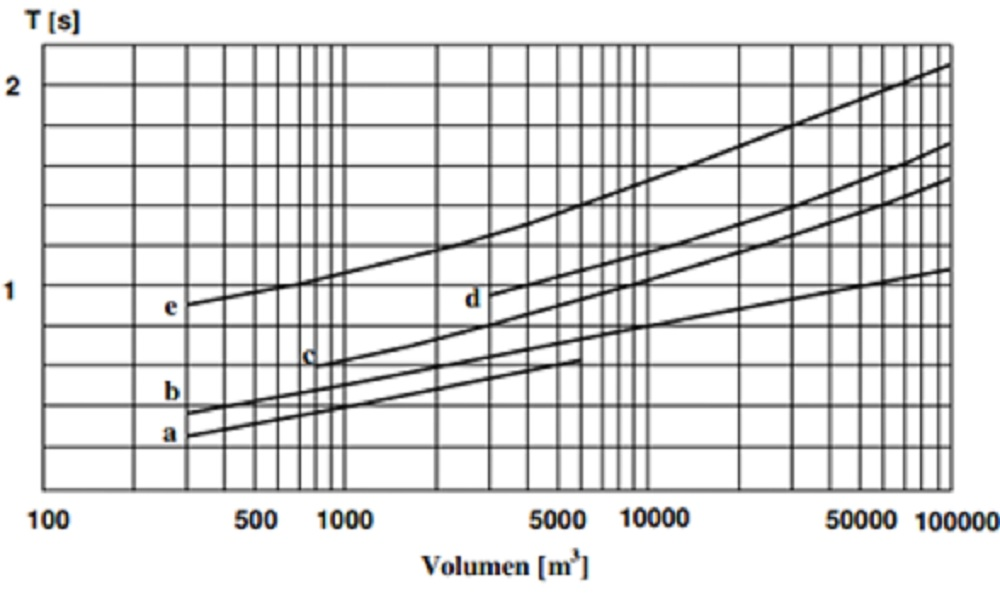
\includegraphics[width=0.7\textwidth]{imagenes/1.jpg}
    \caption{\footnotesize Tiempo de reverberación óptimo en función del volumen de una sala (según L. L. Beranek). (a) Estudios de radiodifusión para voz. (b) Salas de conferencias. (c) Estudios de radiodifusión para música. (d) Salas de conciertos. (e) Iglesias \cite{Miyara2004}.}
    \label{fig:TiempoRevOpt}
\end{figure}
\FloatBarrier

\subsubsection{Resonancias.} Las resonancias o modos normales de vibración suceden como consecuencia de las reflexiones sucesivas en paredes opuestas. Una onda estacionaria es una onda que va y viene una y otra vez entre dos paredes, por lo que, si la distancia entre las dos paredes es L, la longitud de tal onda es 2L y por consiguiente deberá cumplir que

\begin{equation}
2\cdot L = \frac{c}{f}
\end{equation}

Donde c es la velocidad del sonido, y f la frecuencia del sonido resultante. De aquí se puede obtener la frecuencia, que resulta ser

\begin{equation}
f = \frac{c}{2\cdot L}
\end{equation}

Para las frecuencias de resonancia el tiempo de reverberación es mucho más prolongado, por lo cual dicha nota se prolongará más que las otras. Esto se considera un defecto acústico importante. Entre las posibles soluciones, están: a) evitar las superficies paralelas, que favorecen las resonancias, b) agregar absorción acústica que reduzca el tiempo de reverberación, c) ecualizar el sistema de sonido de modo de atenuar las frecuencias próximas a la resonancia o resaltar las otras frecuencias \cite{Miyara2004}.

\subsubsection{Claridad.} La claridad describe el grado en que cada detalle de las actuaciones puede ser percibido en lugar de que todo se difumine por los componentes de sonido reverberantes que llegan más tarde. Por lo tanto, la claridad es en gran medida una propiedad complementaria a la reverberancia.

Cuando las reflexiones se retrasan no más de 50-80 ms en relación con el sonido directo, el oído integrará estas contribuciones y el sonido directo, lo que significa que percibimos principalmente el efecto como si el sonido claro y original se hubiera amplificado en relación con la energía reverberante posterior. Por lo tanto, se ha encontrado que un parámetro objetivo que compara la relación entre la energía en la respuesta al impulso antes y después de 80 ms es un descriptor razonablemente bueno de claridad.

\begin{equation}
C = 10\log_{10}\left[{\frac{\int_0^{80ms} h^2(t) \mathrm{d}t}{\int_{80ms}^{\infty} h^2(t) \mathrm{d}t}}\right]
\end{equation}

Cuanto mayor sea el valor de C, más dominará el sonido inicial y mayor será la impresión de claridad \cite{Rossing2007}.

\subsubsection{Potencia sonora} La influencia de la sala en la sonoridad percibida es otro aspecto importante de la acústica de la sala. Una medida relevante de esta propiedad es simplemente la diferencia en dB entre el nivel de una fuente de sonido continua y calibrada medido en la habitación y el nivel que genera la misma fuente a 10 m de distancia en un entorno anecoico. Esta medida objetiva, denominada fuerza (relativa) G, también puede obtenerse a partir de registros de respuesta al impulso a partir de la relación entre la energía total de la respuesta al impulso y la energía del sonido directo, y esta última se registra a una distancia fija (10 m) de la fuente de sonido impulsivo:

\begin{equation}
G = 10\log_{10}\left[{\frac{\int_0^{\infty} h^2(t) \mathrm{d}t}{\int_0^{t_{dir}} h^2_{10m}(t) \mathrm{d}t}}\right]
\end{equation}

En este caso, el límite superior de integración en el denominador $t_{dir}$ debe limitarse a la duración del impulso de sonido directo (que en la práctica dependerá de la anchura de banda seleccionada). Se puede utilizar una distancia diferente de 10 m, si también se aplica una corrección para la atenuación de la distancia. 

El valor esperado de G según la teoría de campos difusos se convierte en una función de T, así como del volumen de la habitación, V \cite{Rossing2007}:

\begin{equation}
G_{exp} = 10\log_{10}\left({\frac{T}{V}}\right) + 45 dB
\end{equation}

\subsubsection{Medidas de amplitud} La amplitud es la sensación de que el sonido llega desde muchas direcciones diferentes en contraste con una impresión monofónica de todo el sonido que llega al oyente a través de una abertura estrecha. Ahora está claro que hay dos aspectos de la amplitud, los cuales son atractivos, especialmente cuando se escucha música:

Anchura aparente de la fuente (ASW): la impresión de que la imagen sonora es más amplia que la extensión visual y física de la(s) fuente(s) en el escenario. Envolvente del oyente (LEV): la impresión de estar dentro y rodeado por el campo sonoro reverberante de la habitación.

Se ha encontrado que ambos aspectos dependen de la dirección de incidencia de las 
reflexiones de respuesta al impulso. Cuando una mayor parte de la energía de reflexión temprana (hasta unos 80 ms) llega desde direcciones laterales (desde los lados), el ASW aumenta. Cuando el nivel de las reflexiones laterales tardías es alto, se produce un fuerte LEV.

Los componentes laterales de la energía de respuesta al impulso se pueden grabar utilizando un micrófono en forma de ocho con el eje sensible mantenido horizontal y perpendicular a la dirección hacia la fuente de sonido (de modo que la fuente se encuentre en el plano sordo del micrófono). Para la medición de la fracción de energía lateral (LEF), la parte inicial (hasta 80 ms) de esta energía sonora lateral se compara con la energía del sonido directo más todas las reflexiones tempranas captadas por un micrófono omnidireccional ordinario

\begin{equation}
LEF = \frac{\int_{t=5ms}^{t=80ms} h^2_1(t) \mathrm{d}t}{\int_{t=0ms}^{t=80ms} h^2(t) \mathrm{d}t}
\end{equation}

donde $h_1$ es la presión de respuesta al impulso registrada con un micrófono en forma de ocho, mientras que h se captura a través del micrófono omnidireccional (habitual). Es principalmente la energía a frecuencias bajas y medias la que contribuye a la amplitud. En consecuencia, LEF se promedia normalmente en las cuatro octavas 125-1000 Hz. Cuanto mayor sea el valor de LEF, más amplio será el ASW. En un campo completamente difuso, LEF sería constante con 
un valor de 0,33, que es superior al que normalmente se encuentra en las salas reales. La diferencia subjetiva para LEF es de aproximadamente el 5\%. El aspecto ASW de la amplitud no solo depende de la relación entre el sonido lateral temprano y el sonido temprano total; pero también en el nivel total del sonido. Cuanto mayor sea el valor G (y más fuerte sea la fuente de sonido), más amplia será la imagen acústica de la fuente. Sin embargo, en el momento de escribir este artículo, no existe una forma sólida de incorporar la influencia del nivel en la medida objetiva. La envolvente del oyente parece estar determinada principalmente por la distribución espacial y el nivel de las reflexiones tardías (que llegan después de 80 ms) \cite{Rossing2007}.

\subsubsection{Parámetros relacionados con el timbre o el color tonal} El timbre describe el grado en que la habitación influye en el equilibrio de frecuencias entre las frecuencias altas, medias y bajas, es decir, si el sonido es áspero, brillante, hueco, cálido o cualquier otro adjetivo que se use para describir el color tonal. Tradicionalmente, se ha utilizado un gráfico de la variación de frecuencia de T (por 1/1 o 1/3 de octava) para indicar esta cualidad; pero se ha sugerido un conveniente parámetro de un solo número destinado a medir la calidez de la sala: la relación de graves (BR) dada por:

\begin{equation}
BR = \frac{T_{125Hz}+T_{250Hz}}{T_{500Hz}+T_{1000Hz}}
\end{equation}

Del mismo modo, una relación de agudos (TR) se puede formar como:

\begin{equation}
BR = \frac{T_{2000Hz}+T_{4000Hz}}{T_{500Hz}+T_{1000Hz}}
\end{equation}

Sin embargo, en algunas salas, se experimenta una falta de sonido de graves a pesar de los altos valores de T en las frecuencias bajas. Por lo tanto, EDT o tal vez G versus frecuencia sería un parámetro mejor, e intuitivamente más lógico, para la medición del timbre. Del mismo modo, BR o TR podrían basarse en valores G en lugar de T \cite{Rossing2007}.

\subsubsection{Inteligibilidad del habla} Todos los parámetros objetivos mencionados anteriormente (excepto el parámetro básico T), son principalmente relevantes en auditorios más grandes destinados a la interpretación de música. En los auditorios utilizados para el habla, como las salas de conferencias o los teatros, la influencia de la acústica en la inteligibilidad es un problema importante. Actualmente, la forma más común de evaluar objetivamente la inteligibilidad del habla en las salas es mediante la medición del índice de transmisión del habla ST \cite{Rossing2007}.

%Imagen 2
\begin{figure}[!htb]
    \centering
    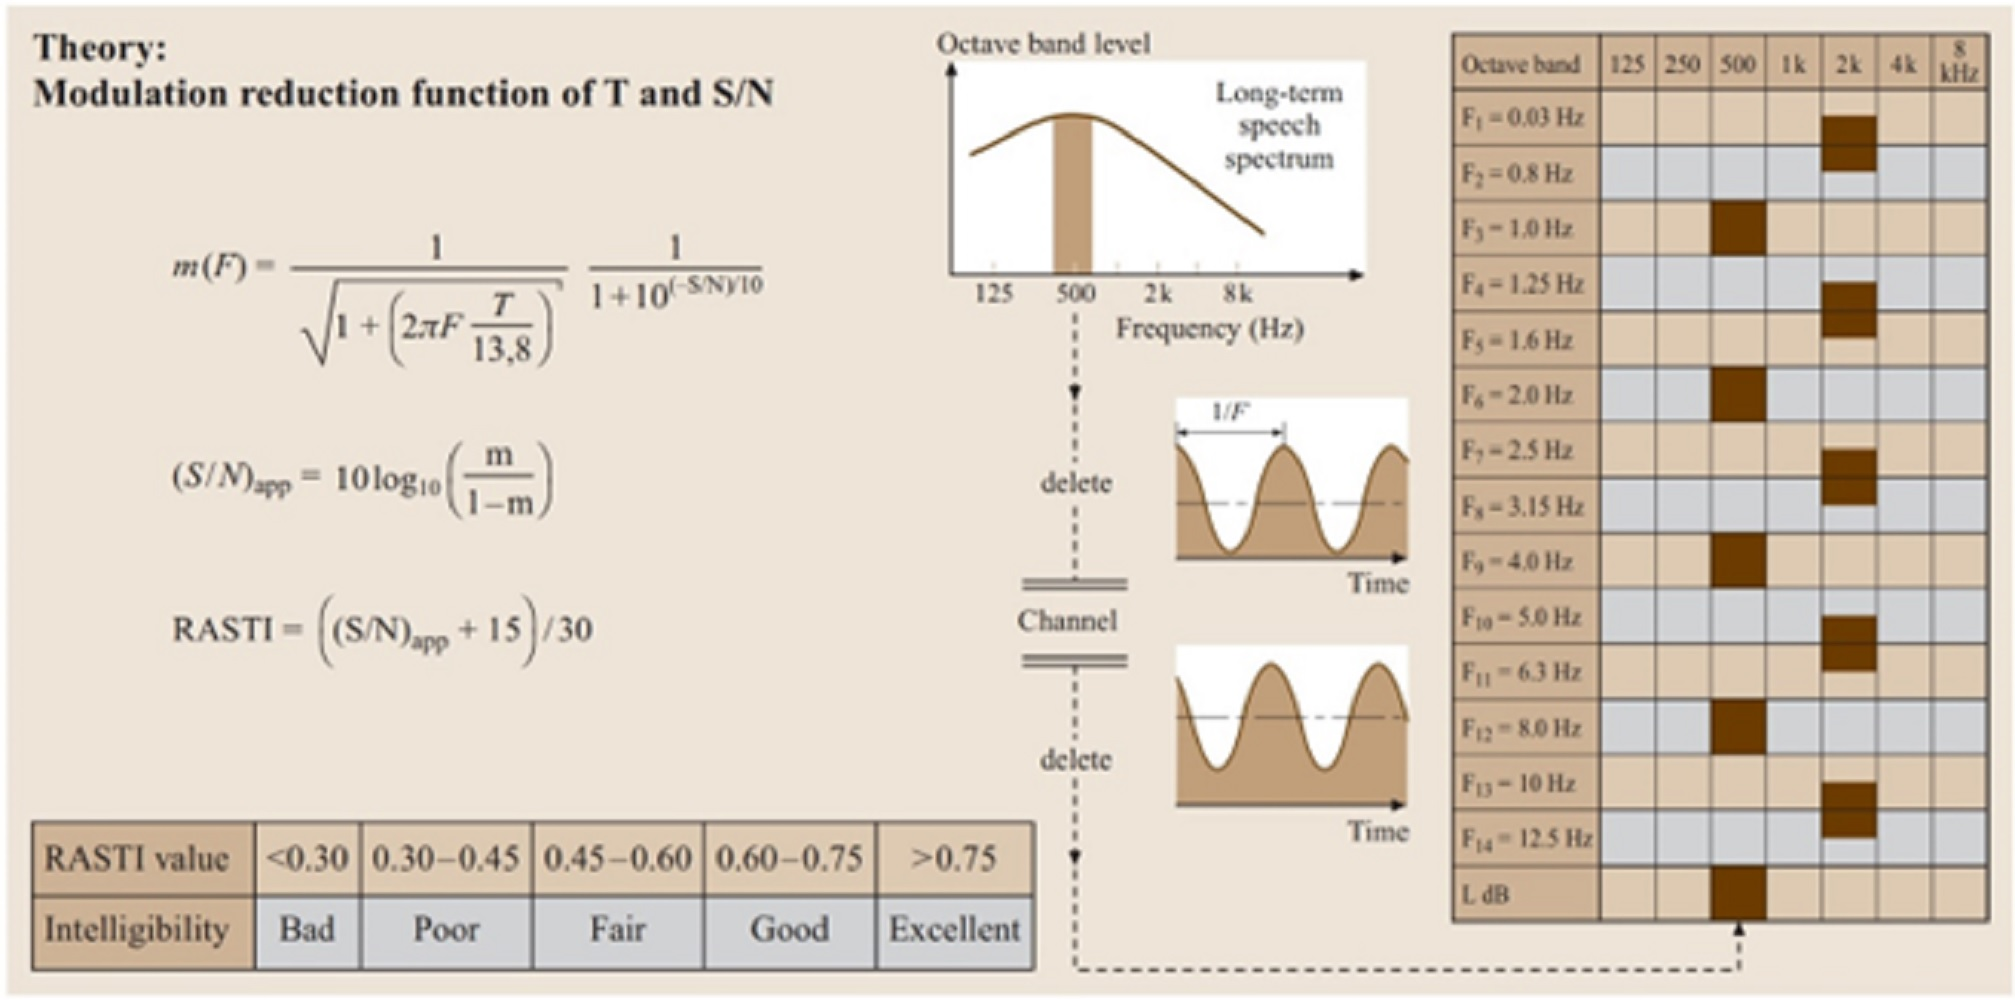
\includegraphics[width=0.9\textwidth]{imagenes/2.jpg}
    \caption{\footnotesize Ilustración de la teoría y el principio en la medición de STI o RASTI. La escala para la evolución de los valores RASTI se muestra en la parte inferior \cite{Rossing2007}.}
    \label{fig:IntelHabla}
\end{figure}
\FloatBarrier

%\addcontentsline{toc}{section}{Propuesta de soluci\'on}
%\section*{Propuesta de soluci\'on}
%\addcontentsline{toc}{subsection}{Definición de la metodología}
\subsection{Marco Precedimental}

\subsubsection{Definici\'on de la metodolog\'ia mecatr\'onica}

La mecatrónica es una ingeniería interdisciplinaria y, por tanto, es necesario buscar 
metodologías de diseño que nos permita especificar las necesidades del sistema, planear actividades, dividir tareas y validar resultados.
\\
En \cite{Geusemeir2002} se muestra la metodología mecatrónica ‘VDI 2206”. En ella se sigue un modelo 
procedimental flexible basado en tres elementos principales:
\begin{itemize}
    \item El ciclo general de resolución de problemas a pequeña escala (micro-level)
    \item El modelo en forma de V en la gran escala (macro-level)
    \item Módulo de procesos predefinidos para pasos de operación que se repiten durante el diseño de los sistemas mecatrónicos.
\end{itemize}

\subsubsection{Resolución de problemas en el micro-level}
La resolución de problemas en el micro-level comienza de dos maneras: analizando la situación actual y analizando la relación de la condición actual con la condición meta. Lo anterior nos lleva a una síntesis y análisis que permite generar, rechazar y elegir soluciones. El análisis de la solución y la evaluación nos puede llevar a replantear la meta o a volver a analizar la situación. Si el resultado es satisfactorio nos sirve como herramienta de aprendizaje y se planean las acciones futuras. \\
El flujo de esta metodología de resolución de problemas se puede ver en la figura \ref{fig:DiagramaMicroLevel}:
%---------------------------------Imagen 3---------------------------------
\begin{figure}[!htb]
    \centering
    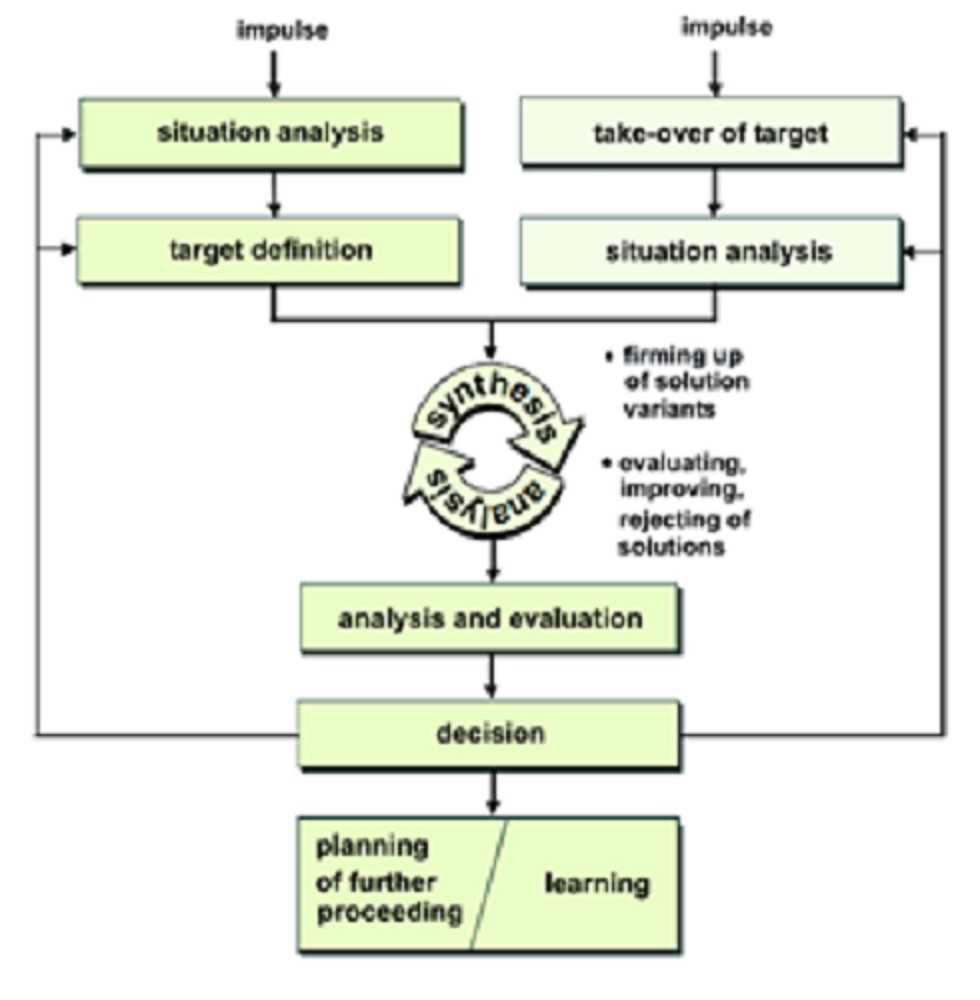
\includegraphics[width=0.6\textwidth]{imagenes/3.jpg}
    \caption{Diagrama de flujo para la resolución de problemas en el micro-level.}
    \label{fig:DiagramaMicroLevel}
\end{figure}
\FloatBarrier
%---------------------------------Imagen 3---------------------------------

\subsubsection{Modelo en V en el macro-level}
En modelo en V, en donde la primera parte es un procedimiento de arriba hacia abajo y la segunda parte es de abajo hacia arriba, nos permitirá separar las tareas a gran escala y realizar validaciones constantes de los sistemas.\\
El modelo V busca partir de los requerimientos y realizar un diseño del sistema conceptual, el cual es multidominio y describe las características esenciales del producto. A continuación, hace diseños específicos para cada dominio, los cuales integra en una etapa posterior y analiza sus interrelaciones. A lo largo de este proceso se debe hacer una verificación y validación constante de que el diseño cumpla con los requerimientos y el diseño conceptual del producto, además de apoyarse en el modelado y la simulación por computadora para hacer estas validaciones. En caso de cumplirse con esto se cuenta con un producto que cumple con los requisitos.\\
El modelo V es un modelo iterativo, es decir, es poco probable que el primer producto al que se llegue después de la integración sea totalmente funcional o incluso el óptimo. Por lo anterior, se deben llevar a cabo múltiples ciclos de diseño y validación, para que el producto alcance un mayor grado de madurez. Cada etapa tiene un “contraparte” a la que se puede volver en caso de que no se cumpla alguna verificación, esto lleva a mejorar el diseño y analizar múltiples opciones de solución.
%---------------------------------Imagen 4---------------------------------
\begin{figure}[!htb]
    \centering
    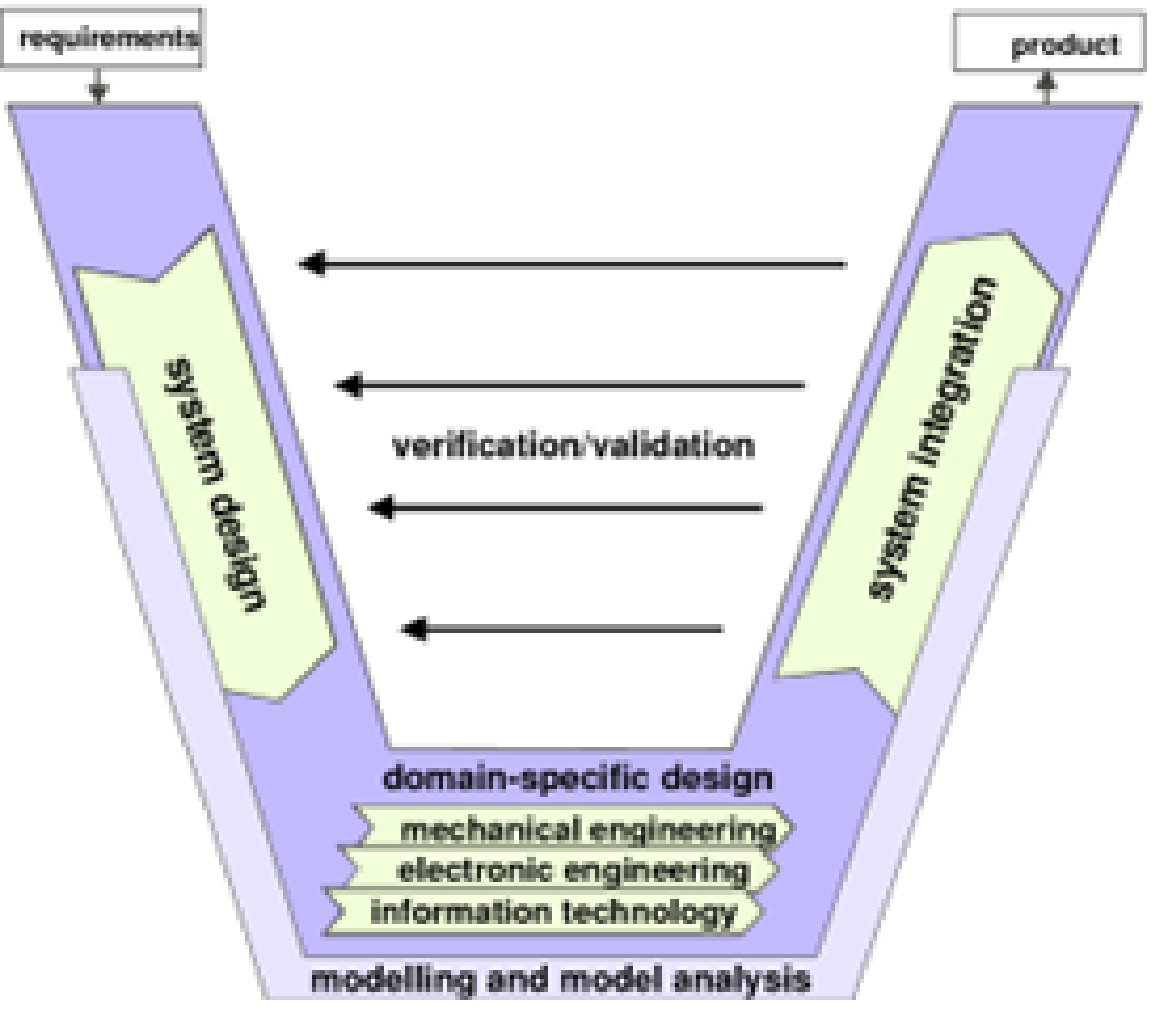
\includegraphics[width=0.5\textwidth]{imagenes/4.jpg}
    \caption{\footnotesize Metodología por seguir.}
    \label{Fig:MetodologiaV}
\end{figure}
\FloatBarrier
%---------------------------------Imagen 4---------------------------------

\subsubsection{Procesos predefinidos}
En cada una de las etapas de diseño, se tienen procesos predefinidos que se repiten regularmente durante estas etapas. Cada uno de estos procesos están mejor definidos en \cite{Pahl1996} y se utilizarán en el desarrollo de este proyecto para la generación de soluciones.

%---------------Media 2---------------
\input{Secciones/Media 2/DiseñoConceptual}
%\definecolor{gr_l}{gray}{.8}
%-----------------------------Matriz Morfológica-----------------------------
\begin{center}
\scriptsize
\centering
    \begin{longtable}[!htb]{|>{\centering\arraybackslash}m{3em} ||>{\centering\arraybackslash}m{8em} | >{\centering\arraybackslash}m{8em}| >{\centering\arraybackslash}m{8em}| >{\centering\arraybackslash}m{8em}|>{\centering\arraybackslash}m{8em}|}
    \hline
    & \textbf{Características} & \textbf{Alternativa 1} & \textbf{Alternativa 2}& \textbf{Alternativa 3}& \textbf{Alternativa 4}\\
    \hline\hline
    \textbf{$C_1$} & Forma de movimiento de los paneles & Rotacional en base prismática & Tipo pick and place & Construcción y movimiento de líneas & Paneles en configuración plegable\\
    \hline
    \textbf{$C_2$} & Método para la reflexión & Paneles de reflexión & Pared de fondo & - & -\\
    \hline
    \textbf{$C_3$} & Grabación en varias posiciones & No & Manual & Automático & Con múltiples micrófonos\\
    \hline
    \textbf{$C_4$} & Generación de ondas de sonido & Bocina de equipo de cómputo & Bocina externa & Bocina para circuitos & - \\
    \hline
    \textbf{$C_5$} & Dispositivo de grabación & Micrófono de equipo de cómputo & Micrófono externo & Micrófono para circuitos & - \\
    \hline
    \textbf{$C_6$} & Plataforma de cálculo para las posiciones deseadas & Equipo de cómputo & Microcontrolador embebido & FPGA & - \\
    \hline
    \textbf{$C_7$} & Plataforma de procesado del control & Equipo de cómputo & Microcontrolador embebido & FPGA & - \\
    \hline
    \textbf{$C_8$} & Plataforma para procesado de la acústica & Equipo de cómputo & Microcontrolador embebido & FPGA & - \\
    \hline
    \textbf{$C_9$} & Sensado de las posiciones de los paneles & Encoders & Sensores de contacto & Visión artificial & Sensor de flexión \\
    \hline
    \textbf{$C_{10}$} & Plataforma de visualización de información & Equipo de cómputo & Pantalla OLED & Pantalla LCD & - \\
    \hline
    \textbf{$C_{11}$} & Control de interfaz & Pantalla táctil & Botonera & Ratón y teclado & - \\
    \hline
    \textbf{$C_{12}$} & Encapsulado de sistemas embebidos & Si & No & - & - \\
    \hline
    \textbf{$C_{13}$} & Inclusión del sistema energético en el sistema embebido & Si & No & - & - \\
    \hline
    \textbf{$C_{14}$} & Anclaje al suelo & Si & No & - & - \\
    \hline
    \textbf{$C_{15}$} & Método de anclaje & Tornillos & Colgados & Adhesivos & Magnéticos \\
    \hline
    \textbf{$C_{16}$} & Método de comunicación & Serial & Wi-fi & Bluetooth & - \\
    \hline

    \caption{Matriz morfológica}
    \label{tab:Matriz morfológica}
    \end{longtable}
\end{center}
%-----------------------------Matriz Morfológica-----------------------------

En base a las diferentes alternativas, se crearon 4 conceptos de solución, cuya mayor diferencia es el método de movimiento para los paneles. Debido a que hay alternativas que no son dependientes del método de movimiento, la selección de estas se hará independientemente. 
%-----------------------------Conceptos solución-----------------------------
\begin{center}
\scriptsize
\centering
    \begin{longtable}[!htb]{|>{\centering\arraybackslash}m{3em} ||>{\centering\arraybackslash}m{8em} | >{\centering\arraybackslash}m{8em}| >{\centering\arraybackslash}m{8em}| >{\centering\arraybackslash}m{8em}|>{\centering\arraybackslash}m{8em}|}
    \hline
    & \textbf{Características} & \textbf{$CS_1$} & \textbf{$CS_2$}& \textbf{$CS_3$}& \textbf{$CS_4$}\\
    \hline\hline
    \textbf{$C_1$} & Forma de movimiento de los paneles & Rotacional en base prismática & Tipo pick and place & Construcción y movimiento de líneas & Paneles en configuración plegable\\
    \hline
    \textbf{$C_2$} & Tipo de actuación & Con motor y acopladores magnéticos & Con motor y actuador magnético & Con motores & Motores lineales\\
    \hline
    \textbf{$C_3$} & Sensado de las posiciones de los paneles & Encoders, sensores de contacto o visión artificial & Encoders o visión artificial & Encoders & Sensores de flexión\\
    \hline
    \textbf{$C_4$} & Posicionamiento de paneles & Anclados a la base prismática & Acoplamiento en pared & Acoplado a un cable & Acoplados entre si\\
    \hline
    \textbf{$C_5$} & Sistema de alimentación de paneles & No & Si & Si & No \\
    \hline

    \caption{Conceptos solución}
    \label{tab:ConceptosSolucion}
    \end{longtable}
\end{center}
%-----------------------------Conceptos solución---------------------------------
Primero se hará la comparación de los diferentes conceptos solución con base en cada uno de los criterios. Es importante notar que no todos los criterios se pueden aplicar para discernir entre los diferentes conceptos solución, por tanto, esos criterios se aplicaran a las alternativas que se analizaran individualmente.
%-------------------------CR1 Velocidad de actuación-----------------------------
\begin{table}[!htbp]
    \begin{minipage}[b]{0.5\linewidth}
        \scriptsize
        \centering
            \begin{tabular}{|>{\centering\arraybackslash}m{2em} ||>{\centering\arraybackslash}m{2em} | >{\centering\arraybackslash}m{2em}| >{\centering\arraybackslash}m{2em}| >{\centering\arraybackslash}m{2em}|}
            \hline
            & \textbf{$CS_1$} & \textbf{$CS_2$}& \textbf{$CS_3$}& \textbf{$CS_4$}\\
            \hline\hline
            \textbf{$CS_1$} & \cellcolor{gr_l}{1}  &  10  &    5   &   2    \\
            \textbf{$CS_2$} & 0.10 &  \cellcolor{gr_l}{1} &  0.50  &  0.20  \\
            \textbf{$CS_3$} & 0.20 &  2   &  \cellcolor{gr_l}{1}   &  0.40  \\
            \textbf{$CS_4$} & 0.50 &  5   &  2.50  &   \cellcolor{gr_l}{1}  \\ 
            \hline
        \end{tabular}
        \caption{Matriz de comparación de $Cr_1$}
        \label{tab:MComCr1}
    \end{minipage}
    \begin{minipage}[b]{0.5\linewidth}
        \scriptsize
        \centering
            \begin{tabular}{|>{\centering\arraybackslash}m{2em} ||>{\centering\arraybackslash}m{2em} | >{\centering\arraybackslash}m{2em}| >{\centering\arraybackslash}m{2em}| >{\centering\arraybackslash}m{2em}|>{\centering\arraybackslash}m{2em}|}
            \hline
            & \textbf{$CS_1$} & \textbf{$CS_2$}& \textbf{$CS_3$}& \textbf{$CS_4$}& \textbf{$V_{Cr_1}$}\\
            \hline\hline
            \textbf{$CS_1$} & 0.56 &  0.56  &   0.56   &  0.56  &  0.56   \\
            \textbf{$CS_2$} & 0.06 &  0.06  &   0.06   &  0.06  &  0.06   \\
            \textbf{$CS_3$} & 0.11 &  0.11  &   0.11   &  0.11  &  0.11   \\
            \textbf{$CS_4$} & 0.28 &  0.28  &   0.28   &  0.28  &  0.28   \\ 
            \hline
        \end{tabular}
        \caption{Matriz normalizada de $Cr_1$ y $V_{Cr_1}$}
        \label{tab:MNorm_Cr1}
    \end{minipage}
\end{table}
%-------------------------CR1 Velocidad de actuación-----------------------------

%-------------------------CR2 Peso-----------------------------
\begin{table}[!htbp]
    \begin{minipage}[b]{0.5\linewidth}
        \scriptsize
        \centering
            \begin{tabular}{|>{\centering\arraybackslash}m{2em} ||>{\centering\arraybackslash}m{2em} | >{\centering\arraybackslash}m{2em}| >{\centering\arraybackslash}m{2em}| >{\centering\arraybackslash}m{2em}|}
            \hline
            & \textbf{$CS_1$} & \textbf{$CS_2$}& \textbf{$CS_3$}& \textbf{$CS_4$}\\
            \hline\hline
            \textbf{$CS_1$} & \cellcolor{gr_l}{1} &  0.38  &  0.38   &   1   \\
            \textbf{$CS_2$} & 2.67 &  \cellcolor{gr_l}{1}  &   1     &  2.67  \\
            \textbf{$CS_3$} & 2.67 &  1      &  \cellcolor{gr_l}{1}   &  2.67  \\
            \textbf{$CS_4$} &   1  &  0.38   &  0.38  &   \cellcolor{gr_l}{1}  \\ 
            \hline
        \end{tabular}
        \caption{Matriz de comparación de $Cr_2$}
        \label{tab:MComCr2}
    \end{minipage}
    \begin{minipage}[b]{0.5\linewidth}
        \scriptsize
        \centering
            \begin{tabular}{|>{\centering\arraybackslash}m{2em} ||>{\centering\arraybackslash}m{2em} | >{\centering\arraybackslash}m{2em}| >{\centering\arraybackslash}m{2em}| >{\centering\arraybackslash}m{2em}|>{\centering\arraybackslash}m{2em}|}
            \hline
            & \textbf{$CS_1$} & \textbf{$CS_2$}& \textbf{$CS_3$}& \textbf{$CS_4$}& \textbf{$V_{Cr_2}$}\\
            \hline\hline
            \textbf{$CS_1$} & 0.14 &  0.14  &   0.14   &  0.14  &  0.14   \\
            \textbf{$CS_2$} & 0.36 &  0.36  &   0.36   &  0.36  &  0.36   \\
            \textbf{$CS_3$} & 0.36 &  0.36  &   0.36   &  0.36  &  0.36   \\
            \textbf{$CS_4$} & 0.14 &  0.14  &   0.14   &  0.14  &  0.14   \\ 
            \hline
        \end{tabular}
        \caption{Matriz normalizada de $Cr_2$ y $V_{Cr_2}$}
        \label{tab:MNorm_Cr1}
    \end{minipage}
\end{table}
%-------------------------CR2 Peso-----------------------------

%-------------------------CR3 Complejidad de mecanismo-----------------------------
\begin{table}[!htbp]
    \begin{minipage}[b]{0.5\linewidth}
        \scriptsize
        \centering
            \begin{tabular}{|>{\centering\arraybackslash}m{2em} ||>{\centering\arraybackslash}m{2em} | >{\centering\arraybackslash}m{2em}| >{\centering\arraybackslash}m{2em}| >{\centering\arraybackslash}m{2em}|}
            \hline
            & \textbf{$CS_1$} & \textbf{$CS_2$}& \textbf{$CS_3$}& \textbf{$CS_4$}\\
            \hline\hline
            \textbf{$CS_1$} & \cellcolor{gr_l}{1}  &  2.67  &    4   &   4   \\
            \textbf{$CS_2$} & 0.38 &  \cellcolor{gr_l}{1} &  1.50   &  1.50  \\
            \textbf{$CS_3$} & 0.25 &  0.67   &  \cellcolor{gr_l}{1}   &  1  \\
            \textbf{$CS_4$} & 0.25 &  0.67   &  1  &   \cellcolor{gr_l}{1}  \\ 
            \hline
        \end{tabular}
        \caption{Matriz de comparación de $Cr_3$}
        \label{tab:MComCr3}
    \end{minipage}
    \begin{minipage}[b]{0.5\linewidth}
        \scriptsize
        \centering
            \begin{tabular}{|>{\centering\arraybackslash}m{2em} ||>{\centering\arraybackslash}m{2em} | >{\centering\arraybackslash}m{2em}| >{\centering\arraybackslash}m{2em}| >{\centering\arraybackslash}m{2em}|>{\centering\arraybackslash}m{2em}|}
            \hline
            & \textbf{$CS_1$} & \textbf{$CS_2$}& \textbf{$CS_3$}& \textbf{$CS_4$}& \textbf{$V_{Cr_3}$}\\
            \hline\hline
            \textbf{$CS_1$} & 0.53 &  0.53  &   0.53   &  0.53  &  0.53   \\
            \textbf{$CS_2$} & 0.20 &  0.20  &   0.20   &  0.20  &  0.20   \\
            \textbf{$CS_3$} & 0.13 &  0.13  &   0.13   &  0.13  &  0.13   \\
            \textbf{$CS_4$} & 0.13 &  0.13  &   0.13   &  0.13  &  0.13   \\ 
            \hline
        \end{tabular}
        \caption{Matriz normalizada de $Cr_3$ y $V_{Cr_3}$}
        \label{tab:MNorm_Cr3}
    \end{minipage}
\end{table}
%-------------------------CR3 Complejidad de mecanismo-----------------------------

%-------------------------CR4 Cantidad de actuadores-----------------------------
\begin{table}[!htbp]
    \begin{minipage}[b]{0.5\linewidth}
        \scriptsize
        \centering
            \begin{tabular}{|>{\centering\arraybackslash}m{2em} ||>{\centering\arraybackslash}m{2em} | >{\centering\arraybackslash}m{2em}| >{\centering\arraybackslash}m{2em}| >{\centering\arraybackslash}m{2em}|}
            \hline
            & \textbf{$CS_1$} & \textbf{$CS_2$}& \textbf{$CS_3$}& \textbf{$CS_4$}\\
            \hline\hline
            \textbf{$CS_1$} & \cellcolor{gr_l}{1}  &  1.17  &    1.40   &   3.50   \\
            \textbf{$CS_2$} & 0.86 &  \cellcolor{gr_l}{1} &  1.20   &  3.00  \\
            \textbf{$CS_3$} & 0.71 &  0.83   &  \cellcolor{gr_l}{1}   &  2.50  \\
            \textbf{$CS_4$} & 0.29 &  0.33   &  0.40  &   \cellcolor{gr_l}{1}  \\ 
            \hline
        \end{tabular}
        \caption{Matriz de comparación de $Cr_4$}
        \label{tab:MComCr4}
    \end{minipage}
    \begin{minipage}[b]{0.5\linewidth}
        \scriptsize
        \centering
            \begin{tabular}{|>{\centering\arraybackslash}m{2em} ||>{\centering\arraybackslash}m{2em} | >{\centering\arraybackslash}m{2em}| >{\centering\arraybackslash}m{2em}| >{\centering\arraybackslash}m{2em}|>{\centering\arraybackslash}m{2em}|}
            \hline
            & \textbf{$CS_1$} & \textbf{$CS_2$}& \textbf{$CS_3$}& \textbf{$CS_4$}& \textbf{$V_{Cr_4}$}\\
            \hline\hline
            \textbf{$CS_1$} & 0.35 &  0.35  &   0.35   &  0.35  &  0.35   \\
            \textbf{$CS_2$} & 0.30 &  0.30  &   0.30   &  0.30  &  0.30   \\
            \textbf{$CS_3$} & 0.25 &  0.25  &   0.25   &  0.25  &  0.25   \\
            \textbf{$CS_4$} & 0.10 &  0.10  &   0.10   &  0.10  &  0.10   \\ 
            \hline
        \end{tabular}
        \caption{Matriz normalizada de $Cr_4$ y $V_{Cr_4}$}
        \label{tab:MNorm_Cr4}
    \end{minipage}
\end{table}
%-------------------------CR4 Cantidad de actuadores-----------------------------

%-------------------------CR5 Costo de la actuación-----------------------------
\begin{table}[!htbp]
    \begin{minipage}[b]{0.5\linewidth}
        \scriptsize
        \centering
            \begin{tabular}{|>{\centering\arraybackslash}m{2em} ||>{\centering\arraybackslash}m{2em} | >{\centering\arraybackslash}m{2em}| >{\centering\arraybackslash}m{2em}| >{\centering\arraybackslash}m{2em}|}
            \hline
            & \textbf{$CS_1$} & \textbf{$CS_2$}& \textbf{$CS_3$}& \textbf{$CS_4$}\\
            \hline\hline
            \textbf{$CS_1$} & \cellcolor{gr_l}{1}  &  0.89  &    1.14   &   4   \\
            \textbf{$CS_2$} & 1.13 &  \cellcolor{gr_l}{1} &  1.29   &  4.50  \\
            \textbf{$CS_3$} & 0.88 &  0.78   &  \cellcolor{gr_l}{1}   &  3.50  \\
            \textbf{$CS_4$} & 0.25 &  0.22   &  0.29  &   \cellcolor{gr_l}{1}  \\ 
            \hline
        \end{tabular}
        \caption{Matriz de comparación de $Cr_5$}
        \label{tab:MComCr5}
    \end{minipage}
    \begin{minipage}[b]{0.5\linewidth}
        \scriptsize
        \centering
            \begin{tabular}{|>{\centering\arraybackslash}m{2em} ||>{\centering\arraybackslash}m{2em} | >{\centering\arraybackslash}m{2em}| >{\centering\arraybackslash}m{2em}| >{\centering\arraybackslash}m{2em}|>{\centering\arraybackslash}m{2em}|}
            \hline
            & \textbf{$CS_1$} & \textbf{$CS_2$}& \textbf{$CS_3$}& \textbf{$CS_4$}& \textbf{$V_{Cr_5}$}\\
            \hline\hline
            \textbf{$CS_1$} & 0.31 &  0.31  &   0.31   &  0.31  &  0.31   \\
            \textbf{$CS_2$} & 0.35 &  0.35  &   0.35   &  0.35  &  0.35   \\
            \textbf{$CS_3$} & 0.27 &  0.27  &   0.27   &  0.27  &  0.27   \\
            \textbf{$CS_4$} & 0.08 &  0.08  &   0.08   &  0.08  &  0.08   \\ 
            \hline
        \end{tabular}
        \caption{Matriz normalizada de $Cr_5$ y $V_{Cr_5}$}
        \label{tab:MNorm_Cr5}
    \end{minipage}
\end{table}
%-------------------------CR5 Costo de la actuación-----------------------------

%-------------------------CR6 Resolución acústica-----------------------------
\begin{table}[!htbp]
    \begin{minipage}[b]{0.5\linewidth}
        \scriptsize
        \centering
            \begin{tabular}{|>{\centering\arraybackslash}m{2em} ||>{\centering\arraybackslash}m{2em} | >{\centering\arraybackslash}m{2em}| >{\centering\arraybackslash}m{2em}| >{\centering\arraybackslash}m{2em}|}
            \hline
            & \textbf{$CS_1$} & \textbf{$CS_2$}& \textbf{$CS_3$}& \textbf{$CS_4$}\\
            \hline\hline
            \textbf{$CS_1$} & \cellcolor{gr_l}{1}  &  0.90  &    0.90   &   2.25   \\
            \textbf{$CS_2$} & 1.11 &  \cellcolor{gr_l}{1} &  1   &  2.50  \\
            \textbf{$CS_3$} & 1.11 &  1   &  \cellcolor{gr_l}{1}   &  2.50  \\
            \textbf{$CS_4$} & 0.44 &  0.40   &  0.40  &   \cellcolor{gr_l}{1}  \\ 
            \hline
        \end{tabular}
        \caption{Matriz de comparación de $Cr_6$}
        \label{tab:MComCr6}
    \end{minipage}
    \begin{minipage}[b]{0.5\linewidth}
        \scriptsize
        \centering
            \begin{tabular}{|>{\centering\arraybackslash}m{2em} ||>{\centering\arraybackslash}m{2em} | >{\centering\arraybackslash}m{2em}| >{\centering\arraybackslash}m{2em}| >{\centering\arraybackslash}m{2em}|>{\centering\arraybackslash}m{2em}|}
            \hline
            & \textbf{$CS_1$} & \textbf{$CS_2$}& \textbf{$CS_3$}& \textbf{$CS_4$}& \textbf{$V_{Cr_6}$}\\
            \hline\hline
            \textbf{$CS_1$} & 0.27 &  0.27  &   0.27   &  0.27  &  0.27   \\
            \textbf{$CS_2$} & 0.30 &  0.30  &   0.30   &  0.30  &  0.30   \\
            \textbf{$CS_3$} & 0.30 &  0.30  &   0.30   &  0.30  &  0.30    \\
            \textbf{$CS_4$} & 0.12 &  0.12  &   0.12   &  0.12  &  0.12   \\ 
            \hline
        \end{tabular}
        \caption{Matriz normalizada de $Cr_6$ y $V_{Cr_6}$}
        \label{tab:MNorm_Cr6}
    \end{minipage}
\end{table}
%-------------------------CR6 Resolución acústica-----------------------------

%-------------------------CR7 Repetibilidad-----------------------------
\begin{table}[!htbp]
    \begin{minipage}[b]{0.5\linewidth}
        \scriptsize
        \centering
            \begin{tabular}{|>{\centering\arraybackslash}m{2em} ||>{\centering\arraybackslash}m{2em} | >{\centering\arraybackslash}m{2em}| >{\centering\arraybackslash}m{2em}| >{\centering\arraybackslash}m{2em}|}
            \hline
            & \textbf{$CS_1$} & \textbf{$CS_2$}& \textbf{$CS_3$}& \textbf{$CS_4$}\\
            \hline\hline
            \textbf{$CS_1$} & \cellcolor{gr_l}{1}  &  5  &    3.33   &   1.43   \\
            \textbf{$CS_2$} & 0.20 &  \cellcolor{gr_l}{1} &  0.67   &  0.29  \\
            \textbf{$CS_3$} & 0.30 &  1.50   &  \cellcolor{gr_l}{1}   &  0.43  \\
            \textbf{$CS_4$} & 0.70 &  3.50   &  2.33  &   \cellcolor{gr_l}{1}  \\ 
            \hline
        \end{tabular}
        \caption{Matriz de comparación de $Cr_7$}
        \label{tab:MComCr7}
    \end{minipage}
    \begin{minipage}[b]{0.5\linewidth}
        \scriptsize
        \centering
            \begin{tabular}{|>{\centering\arraybackslash}m{2em} ||>{\centering\arraybackslash}m{2em} | >{\centering\arraybackslash}m{2em}| >{\centering\arraybackslash}m{2em}| >{\centering\arraybackslash}m{2em}|>{\centering\arraybackslash}m{2em}|}
            \hline
            & \textbf{$CS_1$} & \textbf{$CS_2$}& \textbf{$CS_3$}& \textbf{$CS_4$}& \textbf{$V_{Cr_7}$}\\
            \hline\hline
            \textbf{$CS_1$} & 0.45 &  0.45  &   0.45   &  0.45  &  0.45   \\
            \textbf{$CS_2$} & 0.09 &  0.09  &   0.09   &  0.09  &  0.09   \\
            \textbf{$CS_3$} & 0.14 &  0.14  &   0.14   &  0.14  &  0.14    \\
            \textbf{$CS_4$} & 0.32 &  0.32  &   0.32   &  0.32  &  0.32   \\ 
            \hline
        \end{tabular}
        \caption{Matriz normalizada de $Cr_7$ y $V_{Cr_7}$}
        \label{tab:MNorm_Cr7}
    \end{minipage}
\end{table}
%-------------------------CR7 Repetibilidad-----------------------------

%-------------------------CR8 Consumo energético-----------------------------
\begin{table}[!htbp]
    \begin{minipage}[b]{0.5\linewidth}
        \scriptsize
        \centering
            \begin{tabular}{|>{\centering\arraybackslash}m{2em} ||>{\centering\arraybackslash}m{2em} | >{\centering\arraybackslash}m{2em}| >{\centering\arraybackslash}m{2em}| >{\centering\arraybackslash}m{2em}|}
            \hline
            & \textbf{$CS_1$} & \textbf{$CS_2$}& \textbf{$CS_3$}& \textbf{$CS_4$}\\
            \hline\hline
            \textbf{$CS_1$} & \cellcolor{gr_l}{1}  &  3  &    2.25   &   4.50   \\
            \textbf{$CS_2$} & 0.33 &  \cellcolor{gr_l}{1} &   0.75   &  1.50  \\
            \textbf{$CS_3$} & 0.44 &  1.33   &  \cellcolor{gr_l}{1}   &  2  \\
            \textbf{$CS_4$} & 0.22 &  0.67   &  0.50  &   \cellcolor{gr_l}{1}  \\ 
            \hline
        \end{tabular}
        \caption{Matriz de comparación de $Cr_8$}
        \label{tab:MComCr8}
    \end{minipage}
    \begin{minipage}[b]{0.5\linewidth}
        \scriptsize
        \centering
            \begin{tabular}{|>{\centering\arraybackslash}m{2em} ||>{\centering\arraybackslash}m{2em} | >{\centering\arraybackslash}m{2em}| >{\centering\arraybackslash}m{2em}| >{\centering\arraybackslash}m{2em}|>{\centering\arraybackslash}m{2em}|}
            \hline
            & \textbf{$CS_1$} & \textbf{$CS_2$}& \textbf{$CS_3$}& \textbf{$CS_4$}& \textbf{$V_{Cr_8}$}\\
            \hline\hline
            \textbf{$CS_1$} & 0.50 &  0.50  &   0.50   &  0.50  &  0.50   \\
            \textbf{$CS_2$} & 0.17 &  0.17  &   0.17   &  0.17  &  0.17   \\
            \textbf{$CS_3$} & 0.22 &  0.22  &   0.22   &  0.22  &  0.22    \\
            \textbf{$CS_4$} & 0.11 &  0.11  &   0.11   &  0.11  &  0.11   \\ 
            \hline
        \end{tabular}
        \caption{Matriz normalizada de $Cr_8$ y $V_{Cr_8}$}
        \label{tab:MNorm_Cr8}
    \end{minipage}
\end{table}
%-------------------------CR8 Consumo energético-----------------------------

%-------------------------CR9 Variedad de potencias consumidas-----------------------------
\begin{table}[!htbp]
    \begin{minipage}[b]{0.5\linewidth}
        \scriptsize
        \centering
            \begin{tabular}{|>{\centering\arraybackslash}m{2em} ||>{\centering\arraybackslash}m{2em} | >{\centering\arraybackslash}m{2em}| >{\centering\arraybackslash}m{2em}| >{\centering\arraybackslash}m{2em}|}
            \hline
            & \textbf{$CS_1$} & \textbf{$CS_2$}& \textbf{$CS_3$}& \textbf{$CS_4$}\\
            \hline\hline
            \textbf{$CS_1$} & \cellcolor{gr_l}{1}  &  1  &    0.88   &   0.70   \\
            \textbf{$CS_2$} & 1 &  \cellcolor{gr_l}{1} &      0.88   &      0.70  \\
            \textbf{$CS_3$} & 1.14 &  1.14   &  \cellcolor{gr_l}{1}   &  0.80  \\
            \textbf{$CS_4$} & 1.43 &  1.43   &  1.25  &   \cellcolor{gr_l}{1}  \\ 
            \hline
        \end{tabular}
        \caption{Matriz de comparación de $Cr_9$}
        \label{tab:MComCr9}
    \end{minipage}
    \begin{minipage}[b]{0.5\linewidth}
        \scriptsize
        \centering
            \begin{tabular}{|>{\centering\arraybackslash}m{2em} ||>{\centering\arraybackslash}m{2em} | >{\centering\arraybackslash}m{2em}| >{\centering\arraybackslash}m{2em}| >{\centering\arraybackslash}m{2em}|>{\centering\arraybackslash}m{2em}|}
            \hline
            & \textbf{$CS_1$} & \textbf{$CS_2$}& \textbf{$CS_3$}& \textbf{$CS_4$}& \textbf{$V_{Cr_9}$}\\
            \hline\hline
            \textbf{$CS_1$} & 0.22 &  0.22  &   0.22   &  0.22  &  0.22   \\
            \textbf{$CS_2$} & 0.22 &  0.22  &   0.22   &  0.22  &  0.22  \\
            \textbf{$CS_3$} & 0.25 &  0.25  &   0.25   &  0.25  &  0.25    \\
            \textbf{$CS_4$} & 0.31 &  0.31  &   0.31   &  0.31  &  0.31   \\ 
            \hline
        \end{tabular}
        \caption{Matriz normalizada de $Cr_9$ y $V_{Cr_9}$}
        \label{tab:MNorm_Cr9}
    \end{minipage}
\end{table}
%-------------------------CR9 Variedad de potencias consumidas-----------------------------

%----------------------CR10 Facilidad en el control de la actuación--------------------------
\begin{table}[!htbp]
    \begin{minipage}[b]{0.5\linewidth}
        \scriptsize
        \centering
            \begin{tabular}{|>{\centering\arraybackslash}m{2em} ||>{\centering\arraybackslash}m{2em} | >{\centering\arraybackslash}m{2em}| >{\centering\arraybackslash}m{2em}| >{\centering\arraybackslash}m{2em}|}
            \hline
            & \textbf{$CS_1$} & \textbf{$CS_2$}& \textbf{$CS_3$}& \textbf{$CS_4$}\\
            \hline\hline
            \textbf{$CS_1$} & \cellcolor{gr_l}{1}  &  9  &    4.50   &   1.29   \\
            \textbf{$CS_2$} & 0.11 &  \cellcolor{gr_l}{1} &   0.50   &   0.14  \\
            \textbf{$CS_3$} & 0.22 &  2   &  \cellcolor{gr_l}{1}   &  0.29  \\
            \textbf{$CS_4$} & 0.78 &  7   &  3.50  &   \cellcolor{gr_l}{1}  \\ 
            \hline
        \end{tabular}
        \caption{Matriz de comparación de $Cr_{10}$}
        \label{tab:MComCr10}
    \end{minipage}
    \begin{minipage}[b]{0.5\linewidth}
        \scriptsize
        \centering
            \begin{tabular}{|>{\centering\arraybackslash}m{2em} ||>{\centering\arraybackslash}m{2em} | >{\centering\arraybackslash}m{2em}| >{\centering\arraybackslash}m{2em}| >{\centering\arraybackslash}m{2em}|>{\centering\arraybackslash}m{2em}|}
            \hline
            & \textbf{$CS_1$} & \textbf{$CS_2$}& \textbf{$CS_3$}& \textbf{$CS_4$}& \textbf{$V_{Cr_{10}}$}\\
            \hline\hline
            \textbf{$CS_1$} & 0.47 &  0.47  &   0.47   &  0.47  &  0.47   \\
            \textbf{$CS_2$} & 0.05 &  0.05  &   0.05   &  0.05  &  0.05  \\
            \textbf{$CS_3$} & 0.11 &  0.11  &   0.11   &  0.11  &  0.11    \\
            \textbf{$CS_4$} & 0.37 &  0.37  &   0.37   &  0.37  &  0.37   \\ 
            \hline
        \end{tabular}
        \caption{Matriz normalizada de $Cr_{10}$ y $V_{Cr_{10}}$}
        \label{tab:MNorm_Cr10}
    \end{minipage}
\end{table}
%----------------------CR10 Facilidad en el control de la actuación--------------------------

%----------------------CR11 Tamaño--------------------------
\begin{table}[!htbp]
    \begin{minipage}[b]{0.5\linewidth}
        \scriptsize
        \centering
            \begin{tabular}{|>{\centering\arraybackslash}m{2em} ||>{\centering\arraybackslash}m{2em} | >{\centering\arraybackslash}m{2em}| >{\centering\arraybackslash}m{2em}| >{\centering\arraybackslash}m{2em}|}
            \hline
            & \textbf{$CS_1$} & \textbf{$CS_2$}& \textbf{$CS_3$}& \textbf{$CS_4$}\\
            \hline\hline
            \textbf{$CS_1$} & \cellcolor{gr_l}{1}  &  1.60  &    2   &   0.89   \\
            \textbf{$CS_2$} & 0.63 &  \cellcolor{gr_l}{1} &   1.25   &   0.56  \\
            \textbf{$CS_3$} & 0.50 &  0.80   &  \cellcolor{gr_l}{1}   &  0.44  \\
            \textbf{$CS_4$} & 1.13 &  1.80   &  2.25  &   \cellcolor{gr_l}{1}  \\ 
            \hline
        \end{tabular}
        \caption{Matriz de comparación de $Cr_{11}$}
        \label{tab:MComCr11}
    \end{minipage}
    \begin{minipage}[b]{0.5\linewidth}
        \scriptsize
        \centering
            \begin{tabular}{|>{\centering\arraybackslash}m{2em} ||>{\centering\arraybackslash}m{2em} | >{\centering\arraybackslash}m{2em}| >{\centering\arraybackslash}m{2em}| >{\centering\arraybackslash}m{2em}|>{\centering\arraybackslash}m{2em}|}
            \hline
            & \textbf{$CS_1$} & \textbf{$CS_2$}& \textbf{$CS_3$}& \textbf{$CS_4$}& \textbf{$V_{Cr_{11}}$}\\
            \hline\hline
            \textbf{$CS_1$} & 0.31 &  0.31  &   0.31   &  0.31  &  0.31   \\
            \textbf{$CS_2$} & 0.19 &  0.19  &   0.19   &  0.19  &  0.19  \\
            \textbf{$CS_3$} & 0.15 &  0.15  &   0.15   &  0.15  &  0.15    \\
            \textbf{$CS_4$} & 0.35 &  0.35  &   0.35   &  0.35  &  0.35   \\ 
            \hline
        \end{tabular}
        \caption{Matriz normalizada de $Cr_{11}$ y $V_{Cr_{11}}$}
        \label{tab:MNorm_Cr11}
    \end{minipage}
\end{table}
%----------------------CR11 Tamaño--------------------------

%----------------------CR12 Confiabilidad del sistema de actuación--------------------------
\begin{table}[!htbp]
    \begin{minipage}[b]{0.5\linewidth}
        \scriptsize
        \centering
            \begin{tabular}{|>{\centering\arraybackslash}m{2em} ||>{\centering\arraybackslash}m{2em} | >{\centering\arraybackslash}m{2em}| >{\centering\arraybackslash}m{2em}| >{\centering\arraybackslash}m{2em}|}
            \hline
            & \textbf{$CS_1$} & \textbf{$CS_2$}& \textbf{$CS_3$}& \textbf{$CS_4$}\\
            \hline\hline
            \textbf{$CS_1$} & \cellcolor{gr_l}{1}  &  5  &    5   &   2.50   \\
            \textbf{$CS_2$} & 0.20 &  \cellcolor{gr_l}{1} &   1   &   0.50  \\
            \textbf{$CS_3$} & 0.20 &  1   &  \cellcolor{gr_l}{1}   &  0.50  \\
            \textbf{$CS_4$} & 0.40 &  2   &  2  &   \cellcolor{gr_l}{1}  \\ 
            \hline
        \end{tabular}
        \caption{Matriz de comparación de $Cr_{12}$}
        \label{tab:MComCr12}
    \end{minipage}
    \begin{minipage}[b]{0.5\linewidth}
        \scriptsize
        \centering
            \begin{tabular}{|>{\centering\arraybackslash}m{2em} ||>{\centering\arraybackslash}m{2em} | >{\centering\arraybackslash}m{2em}| >{\centering\arraybackslash}m{2em}| >{\centering\arraybackslash}m{2em}|>{\centering\arraybackslash}m{2em}|}
            \hline
            & \textbf{$CS_1$} & \textbf{$CS_2$}& \textbf{$CS_3$}& \textbf{$CS_4$}& \textbf{$V_{Cr_{12}}$}\\
            \hline\hline
            \textbf{$CS_1$} & 0.56 &  0.56  &   0.56   &  0.56  &  0.56   \\
            \textbf{$CS_2$} & 0.11 &  0.11  &   0.11   &  0.11  &  0.11  \\
            \textbf{$CS_3$} & 0.11 &  0.11  &   0.11   &  0.11  &  0.11    \\
            \textbf{$CS_4$} & 0.22 &  0.22  &   0.22   &  0.22  &  0.22   \\ 
            \hline
        \end{tabular}
        \caption{Matriz normalizada de $Cr_{12}$ y $V_{Cr_{12}}$}
        \label{tab:MNorm_Cr12}
    \end{minipage}
\end{table}
%----------------------CR12 Confiabilidad del sistema de actuación--------------------------

%---------------CR13 Complejidad de manufactura del mecanismo de actuación------------------
\begin{table}[!htbp]
    \begin{minipage}[b]{0.5\linewidth}
        \scriptsize
        \centering
            \begin{tabular}{|>{\centering\arraybackslash}m{2em} ||>{\centering\arraybackslash}m{2em} | >{\centering\arraybackslash}m{2em}| >{\centering\arraybackslash}m{2em}| >{\centering\arraybackslash}m{2em}|}
            \hline
            & \textbf{$CS_1$} & \textbf{$CS_2$}& \textbf{$CS_3$}& \textbf{$CS_4$}\\
            \hline\hline
            \textbf{$CS_1$} & \cellcolor{gr_l}{1}  &  2  &    3   &   2   \\
            \textbf{$CS_2$} & 0.50 &  \cellcolor{gr_l}{1} &   1.50   &   1  \\
            \textbf{$CS_3$} & 0.33 &  0.67   &  \cellcolor{gr_l}{1}   &  0.67  \\
            \textbf{$CS_4$} & 0.50 &  1   &  1.50  &   \cellcolor{gr_l}{1}  \\ 
            \hline
        \end{tabular}
        \caption{Matriz de comparación de $Cr_{13}$}
        \label{tab:MComCr13}
    \end{minipage}
    \begin{minipage}[b]{0.5\linewidth}
        \scriptsize
        \centering
            \begin{tabular}{|>{\centering\arraybackslash}m{2em} ||>{\centering\arraybackslash}m{2em} | >{\centering\arraybackslash}m{2em}| >{\centering\arraybackslash}m{2em}| >{\centering\arraybackslash}m{2em}|>{\centering\arraybackslash}m{2em}|}
            \hline
            & \textbf{$CS_1$} & \textbf{$CS_2$}& \textbf{$CS_3$}& \textbf{$CS_4$}& \textbf{$V_{Cr_{13}}$}\\
            \hline\hline
            \textbf{$CS_1$} & 0.43 &  0.43  &   0.43   &  0.43  &  0.43   \\
            \textbf{$CS_2$} & 0.21 &  0.21  &   0.21   &  0.21  &  0.21  \\
            \textbf{$CS_3$} & 0.14 &  0.14  &   0.14   &  0.14  &  0.14    \\
            \textbf{$CS_4$} & 0.21 &  0.21  &   0.21   &  0.21  &  0.21   \\ 
            \hline
        \end{tabular}
        \caption{Matriz normalizada de $Cr_{13}$ y $V_{Cr_{13}}$}
        \label{tab:MNorm_Cr13}
    \end{minipage}
\end{table}
%---------------CR13 Complejidad de manufactura del mecanismo de actuación------------------

%---------------CR14 Error de posición------------------
\begin{table}[!htbp]
    \begin{minipage}[b]{0.5\linewidth}
        \scriptsize
        \centering
            \begin{tabular}{|>{\centering\arraybackslash}m{2em} ||>{\centering\arraybackslash}m{2em} | >{\centering\arraybackslash}m{2em}| >{\centering\arraybackslash}m{2em}| >{\centering\arraybackslash}m{2em}|}
            \hline
            & \textbf{$CS_1$} & \textbf{$CS_2$}& \textbf{$CS_3$}& \textbf{$CS_4$}\\
            \hline\hline
            \textbf{$CS_1$} & \cellcolor{gr_l}{1}  &  10  &    2   &   1.25   \\
            \textbf{$CS_2$} & 0.10 &  \cellcolor{gr_l}{1} &   0.20   &   0.13  \\
            \textbf{$CS_3$} & 0.50 &  5   &  \cellcolor{gr_l}{1}   &  0.63  \\
            \textbf{$CS_4$} & 0.80 &  8   &  1.60  &   \cellcolor{gr_l}{1}  \\ 
            \hline
        \end{tabular}
        \caption{Matriz de comparación de $Cr_{14}$}
        \label{tab:MComCr14}
    \end{minipage}
    \begin{minipage}[b]{0.5\linewidth}
        \scriptsize
        \centering
            \begin{tabular}{|>{\centering\arraybackslash}m{2em} ||>{\centering\arraybackslash}m{2em} | >{\centering\arraybackslash}m{2em}| >{\centering\arraybackslash}m{2em}| >{\centering\arraybackslash}m{2em}|>{\centering\arraybackslash}m{2em}|}
            \hline
            & \textbf{$CS_1$} & \textbf{$CS_2$}& \textbf{$CS_3$}& \textbf{$CS_4$}& \textbf{$V_{Cr_{14}}$}\\
            \hline\hline
            \textbf{$CS_1$} & 0.42 &  0.42  &   0.42   &  0.42  &  0.42   \\
            \textbf{$CS_2$} & 0.04 &  0.04  &   0.04   &  0.04  &  0.04  \\
            \textbf{$CS_3$} & 0.21 &  0.21  &   0.21   &  0.21  &  0.21    \\
            \textbf{$CS_4$} & 0.33 &  0.33  &   0.33   &  0.33  &  0.33   \\ 
            \hline
        \end{tabular}
        \caption{Matriz normalizada de $Cr_{14}$ y $V_{Cr_{14}}$}
        \label{tab:MNorm_Cr14}
    \end{minipage}
\end{table}
%---------------CR14 Error de posición------------------

%---------------CR21 Robustez necesaria del anclaje------------------
\begin{table}[!htbp]
    \begin{minipage}[b]{0.5\linewidth}
        \scriptsize
        \centering
            \begin{tabular}{|>{\centering\arraybackslash}m{2em} ||>{\centering\arraybackslash}m{2em} | >{\centering\arraybackslash}m{2em}| >{\centering\arraybackslash}m{2em}| >{\centering\arraybackslash}m{2em}|}
            \hline
            & \textbf{$CS_1$} & \textbf{$CS_2$}& \textbf{$CS_3$}& \textbf{$CS_4$}\\
            \hline\hline
            \textbf{$CS_1$} & \cellcolor{gr_l}{1}  &  2  &    2   &   1   \\
            \textbf{$CS_2$} & 0.50 &  \cellcolor{gr_l}{1} &   1   &   0.50  \\
            \textbf{$CS_3$} & 0.50 &  1   &  \cellcolor{gr_l}{1}   &  0.50  \\
            \textbf{$CS_4$} & 1 &  2   &  2  &   \cellcolor{gr_l}{1}  \\ 
            \hline
        \end{tabular}
        \caption{Matriz de comparación de $Cr_{21}$}
        \label{tab:MComCr21}
    \end{minipage}
    \begin{minipage}[b]{0.5\linewidth}
        \scriptsize
        \centering
            \begin{tabular}{|>{\centering\arraybackslash}m{2em} ||>{\centering\arraybackslash}m{2em} | >{\centering\arraybackslash}m{2em}| >{\centering\arraybackslash}m{2em}| >{\centering\arraybackslash}m{2em}|>{\centering\arraybackslash}m{2em}|}
            \hline
            & \textbf{$CS_1$} & \textbf{$CS_2$}& \textbf{$CS_3$}& \textbf{$CS_4$}& \textbf{$V_{Cr_{21}}$}\\
            \hline\hline
            \textbf{$CS_1$} & 0.33 &  0.33  &   0.33   &  0.33  &  0.33   \\
            \textbf{$CS_2$} & 0.17 &  0.17  &   0.17   &  0.17  &  0.17  \\
            \textbf{$CS_3$} & 0.17 &  0.17  &   0.17   &  0.17  &  0.17    \\
            \textbf{$CS_4$} & 0.33 &  0.33  &   0.33   &  0.33  &  0.33   \\ 
            \hline
        \end{tabular}
        \caption{Matriz normalizada de $Cr_{21}$ y $V_{Cr_{21}}$}
        \label{tab:MNorm_Cr21}
    \end{minipage}
\end{table}
%---------------CR21 Robustez necesaria del anclaje------------------

%---------------CR22 Propension a fallas estructurales------------------
\begin{table}[!htbp]
    \begin{minipage}[b]{0.5\linewidth}
        \scriptsize
        \centering
            \begin{tabular}{|>{\centering\arraybackslash}m{2em} ||>{\centering\arraybackslash}m{2em} | >{\centering\arraybackslash}m{2em}| >{\centering\arraybackslash}m{2em}| >{\centering\arraybackslash}m{2em}|}
            \hline
            & \textbf{$CS_1$} & \textbf{$CS_2$}& \textbf{$CS_3$}& \textbf{$CS_4$}\\
            \hline\hline
            \textbf{$CS_1$} & \cellcolor{gr_l}{1}  &  7  &    7   &   1   \\
            \textbf{$CS_2$} & 0.14 &  \cellcolor{gr_l}{1} &   1   &   0.14  \\
            \textbf{$CS_3$} & 0.14 &  1   &  \cellcolor{gr_l}{1}   &  0.14  \\
            \textbf{$CS_4$} & 1 &  7   &  7  &   \cellcolor{gr_l}{1}  \\ 
            \hline
        \end{tabular}
        \caption{Matriz de comparación de $Cr_{22}$}
        \label{tab:MComCr22}
    \end{minipage}
    \begin{minipage}[b]{0.5\linewidth}
        \scriptsize
        \centering
            \begin{tabular}{|>{\centering\arraybackslash}m{2em} ||>{\centering\arraybackslash}m{2em} | >{\centering\arraybackslash}m{2em}| >{\centering\arraybackslash}m{2em}| >{\centering\arraybackslash}m{2em}|>{\centering\arraybackslash}m{2em}|}
            \hline
            & \textbf{$CS_1$} & \textbf{$CS_2$}& \textbf{$CS_3$}& \textbf{$CS_4$}& \textbf{$V_{Cr_{22}}$}\\
            \hline\hline
            \textbf{$CS_1$} & 0.44 &  0.44  &   0.44   &  0.44  &  0.44   \\
            \textbf{$CS_2$} & 0.06 &  0.06  &   0.06   &  0.06  &  0.06  \\
            \textbf{$CS_3$} & 0.06 &  0.06  &   0.06   &  0.06  &  0.06    \\
            \textbf{$CS_4$} & 0.44 &  0.44  &   0.44   &  0.44  &  0.44   \\ 
            \hline
        \end{tabular}
        \caption{Matriz normalizada de $Cr_{22}$ y $V_{Cr_{22}}$}
        \label{tab:MNorm_Cr22}
    \end{minipage}
\end{table}
%---------------CR22 Propension a fallas estructurales------------------

%---------------CR24 Facilidad para saltar entre disposiciones------------------
\begin{table}[!htbp]
    \begin{minipage}[b]{0.5\linewidth}
        \scriptsize
        \centering
            \begin{tabular}{|>{\centering\arraybackslash}m{2em} ||>{\centering\arraybackslash}m{2em} | >{\centering\arraybackslash}m{2em}| >{\centering\arraybackslash}m{2em}| >{\centering\arraybackslash}m{2em}|}
            \hline
            & \textbf{$CS_1$} & \textbf{$CS_2$}& \textbf{$CS_3$}& \textbf{$CS_4$}\\
            \hline\hline
            \textbf{$CS_1$} & \cellcolor{gr_l}{1}  &  10  &    5   &   1.25   \\
            \textbf{$CS_2$} & 0.10 &  \cellcolor{gr_l}{1} &   0.50   &   0.13  \\
            \textbf{$CS_3$} & 0.20 &  2   &  \cellcolor{gr_l}{1}   &  0.25  \\
            \textbf{$CS_4$} & 0.80 &  8   &  4  &   \cellcolor{gr_l}{1}  \\ 
            \hline
        \end{tabular}
        \caption{Matriz de comparación de $Cr_{24}$}
        \label{tab:MComCr24}
    \end{minipage}
    \begin{minipage}[b]{0.5\linewidth}
        \scriptsize
        \centering
            \begin{tabular}{|>{\centering\arraybackslash}m{2em} ||>{\centering\arraybackslash}m{2em} | >{\centering\arraybackslash}m{2em}| >{\centering\arraybackslash}m{2em}| >{\centering\arraybackslash}m{2em}|>{\centering\arraybackslash}m{2em}|}
            \hline
            & \textbf{$CS_1$} & \textbf{$CS_2$}& \textbf{$CS_3$}& \textbf{$CS_4$}& \textbf{$V_{Cr_{24}}$}\\
            \hline\hline
            \textbf{$CS_1$} & 0.48 &  0.48  &   0.48   &  0.48  &  0.48   \\
            \textbf{$CS_2$} & 0.05 &  0.05  &   0.05   &  0.05  &  0.05  \\
            \textbf{$CS_3$} & 0.10 &  0.10  &   0.10   &  0.10  &  0.10    \\
            \textbf{$CS_4$} & 0.38 &  0.38  &   0.38   &  0.38  &  0.38   \\ 
            \hline
        \end{tabular}
        \caption{Matriz normalizada de $Cr_{24}$ y $V_{Cr_{24}}$}
        \label{tab:MNorm_Cr24}
    \end{minipage}
\end{table}
%---------------CR24 Facilidad para saltar entre disposiciones------------------

%-------------------CR25 Modularidad----------------------
\begin{table}[!htbp]
    \begin{minipage}[b]{0.5\linewidth}
        \scriptsize
        \centering
            \begin{tabular}{|>{\centering\arraybackslash}m{2em} ||>{\centering\arraybackslash}m{2em} | >{\centering\arraybackslash}m{2em}| >{\centering\arraybackslash}m{2em}| >{\centering\arraybackslash}m{2em}|}
            \hline
            & \textbf{$CS_1$} & \textbf{$CS_2$}& \textbf{$CS_3$}& \textbf{$CS_4$}\\
            \hline\hline
            \textbf{$CS_1$} & \cellcolor{gr_l}{1}  &  4  &    2.67   &   1.33   \\
            \textbf{$CS_2$} & 0.25 &  \cellcolor{gr_l}{1} &   0.67   &   0.33  \\
            \textbf{$CS_3$} & 0.38 &  1.50   &  \cellcolor{gr_l}{1}   &  0.50  \\
            \textbf{$CS_4$} & 0.75 &  3   &  2  &   \cellcolor{gr_l}{1}  \\ 
            \hline
        \end{tabular}
        \caption{Matriz de comparación de $Cr_{25}$}
        \label{tab:MComCr25}
    \end{minipage}
    \begin{minipage}[b]{0.5\linewidth}
        \scriptsize
        \centering
            \begin{tabular}{|>{\centering\arraybackslash}m{2em} ||>{\centering\arraybackslash}m{2em} | >{\centering\arraybackslash}m{2em}| >{\centering\arraybackslash}m{2em}| >{\centering\arraybackslash}m{2em}|>{\centering\arraybackslash}m{2em}|}
            \hline
            & \textbf{$CS_1$} & \textbf{$CS_2$}& \textbf{$CS_3$}& \textbf{$CS_4$}& \textbf{$V_{Cr_{25}}$}\\
            \hline\hline
            \textbf{$CS_1$} & 0.42 &  0.42  &   0.42   &  0.42  &  0.42   \\
            \textbf{$CS_2$} & 0.11 &  0.11  &   0.11   &  0.11  &  0.11  \\
            \textbf{$CS_3$} & 0.16 &  0.16  &   0.16   &  0.16  &  0.16    \\
            \textbf{$CS_4$} & 0.32 &  0.32  &   0.32   &  0.32  &  0.32   \\ 
            \hline
        \end{tabular}
        \caption{Matriz normalizada de $Cr_{25}$ y $V_{Cr_{25}}$}
        \label{tab:MNorm_Cr25}
    \end{minipage}
\end{table}
%-------------------CR25 Modularidad----------------------

%-------------------CR27 Cantidad de paneles utilizados----------------------
\begin{table}[!htbp]
    \begin{minipage}[b]{0.5\linewidth}
        \scriptsize
        \centering
            \begin{tabular}{|>{\centering\arraybackslash}m{2em} ||>{\centering\arraybackslash}m{2em} | >{\centering\arraybackslash}m{2em}| >{\centering\arraybackslash}m{2em}| >{\centering\arraybackslash}m{2em}|}
            \hline
            & \textbf{$CS_1$} & \textbf{$CS_2$}& \textbf{$CS_3$}& \textbf{$CS_4$}\\
            \hline\hline
            \textbf{$CS_1$} & \cellcolor{gr_l}{1}  &  0.57  &    0.57   &   1   \\
            \textbf{$CS_2$} & 1.75 &  \cellcolor{gr_l}{1} &   1   &   1.75  \\
            \textbf{$CS_3$} & 1.75 &  1   &  \cellcolor{gr_l}{1}   &  1.75  \\
            \textbf{$CS_4$} & 1  &   0.57   &  0.57  &   \cellcolor{gr_l}{1}  \\ 
            \hline
        \end{tabular}
        \caption{Matriz de comparación de $Cr_{27}$}
        \label{tab:MComCr27}
    \end{minipage}
    \begin{minipage}[b]{0.5\linewidth}
        \scriptsize
        \centering
            \begin{tabular}{|>{\centering\arraybackslash}m{2em} ||>{\centering\arraybackslash}m{2em} | >{\centering\arraybackslash}m{2em}| >{\centering\arraybackslash}m{2em}| >{\centering\arraybackslash}m{2em}|>{\centering\arraybackslash}m{2em}|}
            \hline
            & \textbf{$CS_1$} & \textbf{$CS_2$}& \textbf{$CS_3$}& \textbf{$CS_4$}& \textbf{$V_{Cr_{27}}$}\\
            \hline\hline
            \textbf{$CS_1$} & 0.18 &  0.18  &   0.18   &  0.18  &  0.18   \\
            \textbf{$CS_2$} & 0.32 &  0.32  &   0.32   &  0.32  &  0.32  \\
            \textbf{$CS_3$} & 0.32 &  0.32  &   0.32   &  0.32  &  0.32    \\
            \textbf{$CS_4$} & 0.18 &  0.18  &   0.18   &  0.18  &  0.18   \\ 
            \hline
        \end{tabular}
        \caption{Matriz normalizada de $Cr_{27}$ y $V_{Cr_{27}}$}
        \label{tab:MNorm_Cr27}
    \end{minipage}
\end{table}
%-------------------CR27 Cantidad de paneles utilizados----------------------
A continuación, y siguiendo la metodología, se deben comparar los criterios de modo que nos permitan obtener un vector de prioridad. Lo anterior es resultado de la diferencia en la importancia que se le asigna a cada criterio. 
%-------------------Matriz de comparacion de criterios----------------------
\begin{landscape}
    \begin{table}[!htb]
    \scriptsize
    \centering
        \begin{tabular}{|>{\centering\arraybackslash}m{2em} ||>{\centering\arraybackslash}m{2em} | >{\centering\arraybackslash}m{2em}| >{\centering\arraybackslash}m{2em}| >{\centering\arraybackslash}m{2em}|>{\centering\arraybackslash}m{2em}|>{\centering\arraybackslash}m{2em}|>{\centering\arraybackslash}m{2em}|>{\centering\arraybackslash}m{2em}|>{\centering\arraybackslash}m{2em}|>{\centering\arraybackslash}m{2em}|>{\centering\arraybackslash}m{2em}|>{\centering\arraybackslash}m{2em}|>{\centering\arraybackslash}m{2em}|>{\centering\arraybackslash}m{2em}|>{\centering\arraybackslash}m{2em}|>{\centering\arraybackslash}m{2em}|>{\centering\arraybackslash}m{2em}|>{\centering\arraybackslash}m{2em}|>{\centering\arraybackslash}m{2em}|} % Especifica las columnas aquí
            \hline
             &$Cr_{1}$ & $Cr_{2}$ & $Cr_{3}$ & $Cr_{4}$ & $Cr_{5}$ & $Cr_{6}$ & $Cr_{7}$ & $Cr_{8}$ & $Cr_{9}$ & $Cr_{10}$ & $Cr_{11}$ & $Cr_{12}$ & $Cr_{13}$ & $Cr_{14}$& $Cr_{21}$ & $Cr_{22}$ & $Cr_{24}$ & $Cr_{25}$ & $Cr_{27}$\\
            \hline
            \hline
            $Cr_{1}$ & \cellcolor{gr_l}{1} & 5 & 0.75 & 3 & 3 & 1 & 3 & 5 & 10 & 5 & 3 & 2 & 5 & 2 & 8 & 2 & 1& 5& 4 \\
            $Cr_{2}$ & 0.20 & \cellcolor{gr_l}{1} & 6.67 & 1.67 & 1.67 & 5 & 1.67 & 1 & 0.50 & 1 & 1.67 & 2.50 & 1 & 2.50 & 0.63 & 2.50 & 5 & 1 & 1.25\\
            $Cr_{3}$ & 1.33 & 0.15 & \cellcolor{gr_l}{1} & 0.25 & 0.25 & 0.75 & 0.25 & 0.15 & 0.08 & 0.15 & 0.25 & 0.38 & 0.15 & 0.38 & 0.09 & 0.38 & 0.75 & 0.15 & 0.19\\
            $Cr_{4}$ & 0.33 & 0.60 & 4 & \cellcolor{gr_l}{1} & 1 & 3 & 1 & 0.60 & 0.30 & 0.60 & 1 & 1.50 & 0.60 & 1.50 & 0.38 & 1.50 & 3 & 0.60 & 0.75\\
            $Cr_{5}$ & 0.33 & 0.60 & 4 & 1 & \cellcolor{gr_l}{1} & 3 & 1 & 0.60 & 0.30 & 0.60 & 1 & 1.50 & 0.60 & 1.50 & 0.38 & 1.50 & 3 & 0.60 & 0.75\\
            $Cr_{6}$ & 1 & 0.20 & 1.33 & 0.33 & 0.33 & \cellcolor{gr_l}{1} & 0.33 & 0.20 & 0.10 & 0.20 & 0.33 & 0.50 & 0.20 & 0.50 & 0.13 & 0.50 & 1 & 0.20 & 0.25\\
            $Cr_{7}$ & 0.33 & 0.60 & 4 & 1 & 1 & 3 & \cellcolor{gr_l}{1} & 0.60 & 0.30 & 0.60 & 1 & 1.50 & 0.60 & 1.50 & 0.38 & 1.50 & 3 & 0.60 & 0.75\\
            $Cr_{8}$ & 0.20 & 1 & 6.67 & 1.67 & 1.67 & 5 & 1.67 & \cellcolor{gr_l}{1} & 0.50 & 1 & 1.67 & 2.50 & 1 & 2.50 & 0.63 & 2.50 & 5 & 1 & 1.25\\
            $Cr_{9}$ & 0.10 & 2 & 13.33 & 3.33 & 3.33 & 10 & 3.33 & 2 & \cellcolor{gr_l}{1} & 2 & 3.33 & 5 & 2 & 5 & 1.25 & 5 & 10 & 2 & 2.50\\
            $Cr_{10}$ & 0.20 & 1 & 6.67 & 1.67 & 1.67 & 5 & 1.67 & 1 & 0.50 & \cellcolor{gr_l}{1} & 1.67 & 2.50 & 1 & 2.50 & 0.63 & 2.50 & 5 & 1 & 1.25\\
            $Cr_{11}$ & 0.33 & 0.60 & 4 & 1 & 1 & 3 & 1 & 0.60 & 0.30 & 0.60 & \cellcolor{gr_l}{1} & 1.50 & 0.60 & 1.50 & 0.38 & 1.50 & 3 & 0.60 & 0.75\\
            $Cr_{12}$ & 0.50 & 0.40 & 2.67 & 0.67 & 0.67 & 2 & 0.67 & 0.40 & 0.20 & 0.40 & 0.67 & \cellcolor{gr_l}{1} & 0.40 & 1 & 0.25 & 1 & 2 & 0.40 & 0.50\\
            $Cr_{13}$ & 0.20 & 1 & 6.67 & 1.67 & 1.67 & 5 & 1.67 & 1 & 0.50 & 1 & 1.67 & 2.50 & \cellcolor{gr_l}{1} & 2.50 & 0.63 & 2.50 & 5 & 1 & 1.25\\
            $Cr_{14}$ & 0.50 & 0.40 & 2.67 & 0.67 & 0.67 & 2 & 0.67 & 0.40 & 0.20 & 0.40 & 0.67 & 1 & 0.40 & \cellcolor{gr_l}{1} & 0.25 & 1 & 2 & 0.40 & 0.50\\
            $Cr_{21}$ & 0.13 & 1.60 & 10.67 & 2.67 & 2.67 & 8 & 2.67 & 1.60 & 0.80 & 1.60 & 2.67 & 4 & 1.60 & 4 & \cellcolor{gr_l}{1} & 4 & 8 & 1.60 & 2\\
            $Cr_{22}$ & 0.50 & 0.40 & 2.67 & 0.67 & 0.67 & 2 & 0.67 & 0.40 & 0.20 & 0.40 & 0.67 & 1 & 0.40 & 1 & 0.25 & \cellcolor{gr_l}{1} & 2 & 0.40 & 0.50\\
            $Cr_{24}$ & 1 & 0.20 & 1.33 & 0.33 & 0.33 & 1 & 0.33 & 0.20 & 0.10 & 0.20 & 0.33 & 0.50 & 0.20 & 0.50 & 0.13 & 0.50 & \cellcolor{gr_l}{1} & 0.20 & 0.25\\
            $Cr_{25}$ & 0.20 & 1 & 6.67 & 1.67 & 1.67 & 5 & 1.67 & 1 & 0.50 & 1 & 1.67 & 2.50 & 1 & 2.50 & 0.63 & 2.50 & 5 & \cellcolor{gr_l}{1} & 1.25\\
            $Cr_{27}$ & 0.25 & 0.80 & 5.33 & 1.33 & 1.33 & 4 & 1.33 & 0.80 & 0.40 & 0.80 & 1.33 & 2 & 0.80 & 2 & 0.50 & 2 & 4 & 0.80 & \cellcolor{gr_l}{1}\\
            % Añade más filas según sea necesario
            \hline
        \end{tabular}
        \caption{Matriz de comparación de criterios}
        \label{tab:MCompCrit}
    \end{table}
%--------------------------------------------------------------------------------------------
    \begin{table}[!htb]
    \scriptsize
    \centering
        \begin{tabular}{|>{\centering\arraybackslash}m{2em} ||>{\centering\arraybackslash}m{2em} | >{\centering\arraybackslash}m{2em}| >{\centering\arraybackslash}m{2em}| >{\centering\arraybackslash}m{2em}|>{\centering\arraybackslash}m{2em}|>{\centering\arraybackslash}m{2em}|>{\centering\arraybackslash}m{2em}|>{\centering\arraybackslash}m{2em}|>{\centering\arraybackslash}m{2em}|>{\centering\arraybackslash}m{2em}|>{\centering\arraybackslash}m{2em}|>{\centering\arraybackslash}m{2em}|>{\centering\arraybackslash}m{2em}|>{\centering\arraybackslash}m{2em}|>{\centering\arraybackslash}m{2em}|>{\centering\arraybackslash}m{2em}|>{\centering\arraybackslash}m{2em}|>{\centering\arraybackslash}m{2em}|>{\centering\arraybackslash}m{2em}|>{\centering\arraybackslash}m{2em}|} % Especifica las columnas aquí
            \hline
             &$Cr_{1}$ & $Cr_{2}$ & $Cr_{3}$ & $Cr_{4}$ & $Cr_{5}$ & $Cr_{6}$ & $Cr_{7}$ & $Cr_{8}$ & $Cr_{9}$ & $Cr_{10}$ & $Cr_{11}$ & $Cr_{12}$ & $Cr_{13}$ & $Cr_{14}$& $Cr_{21}$ & $Cr_{22}$ & $Cr_{24}$ & $Cr_{25}$ & $Cr_{27}$ & $V_{C_r}$\\
            \hline
            \hline
            $Cr_{1}$ & 0.116 & 0.270 & 0.008 & 0.117 & 0.117 & 0.015 & 0.117 & 0.270 & 0.596 & 0.270 & 0.117 & 0.056 & 0.270 & 0.056 & 0.486 & 0.056 & 0.015 & 0.270 & 0.191 & 0.133 \\
            $Cr_{2}$ & 0.023 & 0.054 & 0.073 & 0.065 & 0.065 & 0.073 & 0.065 & 0.054 & 0.030 & 0.054 & 0.065 & 0.070 & 0.054 & 0.070 & 0.038 & 0.070 & 0.073 & 0.054 & 0.060 & 0.064 \\
            $Cr_{3}$ & 0.154 & 0.008 & 0.011 & 0.010 & 0.010 & 0.011 & 0.010 & 0.008 & 0.004 & 0.008 & 0.010 & 0.010 & 0.008 & 0.010 & 0.006 & 0.010 & 0.011 & 0.008 & 0.009 & 0.010 \\
            $Cr_{4}$ & 0.039 & 0.032 & 0.044 & 0.039 & 0.039 & 0.044 & 0.039 & 0.032 & 0.018 & 0.032 & 0.039 & 0.042 & 0.032 & 0.042 & 0.023 & 0.042 & 0.044 & 0.032 & 0.036 & 0.038 \\
            $Cr_{5}$ & 0.039 & 0.032 & 0.044 & 0.039 & 0.039 & 0.044 & 0.039 & 0.032 & 0.018 & 0.032 & 0.039 & 0.042 & 0.032 & 0.042 & 0.023 & 0.042 & 0.044 & 0.032 & 0.036 & 0.038 \\
            $Cr_{6}$ & 0.116 & 0.011 & 0.015 & 0.013 & 0.013 & 0.015 & 0.013 & 0.011 & 0.006 & 0.011 & 0.013 & 0.014 & 0.011 & 0.014 & 0.008 & 0.014 & 0.015 & 0.011 & 0.012 & 0.013 \\
            $Cr_{7}$ & 0.039 & 0.032 & 0.044 & 0.039 & 0.039 & 0.044 & 0.039 & 0.032 & 0.018 & 0.032 & 0.039 & 0.042 & 0.032 & 0.042 & 0.023 & 0.042 & 0.044 & 0.032 & 0.036 & 0.038 \\
            $Cr_{8}$ & 0.023 & 0.054 & 0.073 & 0.065 & 0.065 & 0.073 & 0.065 & 0.054 & 0.030 & 0.054 & 0.065 & 0.070 & 0.054 & 0.070 & 0.038 & 0.070 & 0.073 & 0.054 & 0.060 & 0.064 \\
            $Cr_{9}$ & 0.012 & 0.108 & 0.146 & 0.130 & 0.130 & 0.145 & 0.130 & 0.108 & 0.060 & 0.108 & 0.130 & 0.139 & 0.108 & 0.139 & 0.076 & 0.139 & 0.145 & 0.108 & 0.119 & 0.128 \\
            $Cr_{10}$ & 0.023 & 0.054 & 0.073 & 0.065 & 0.065 & 0.073 & 0.065 & 0.054 & 0.030 & 0.054 & 0.065 & 0.070 & 0.054 & 0.070 & 0.038 & 0.070 & 0.073 & 0.054 & 0.060 & 0.064 \\
            $Cr_{11}$ & 0.039 & 0.032 & 0.044 & 0.039 & 0.039 & 0.044 & 0.039 & 0.032 & 0.018 & 0.032 & 0.039 & 0.042 & 0.032 & 0.042 & 0.023 & 0.042 & 0.044 & 0.032 & 0.036 & 0.038 \\
            $Cr_{12}$ & 0.058 & 0.022 & 0.029 & 0.026 & 0.026 & 0.029 & 0.026 & 0.022 & 0.012 & 0.022 & 0.026 & 0.028 & 0.022 & 0.028 & 0.015 & 0.028 & 0.029 & 0.022 & 0.024 & 0.026 \\
            $Cr_{13}$ & 0.023 & 0.054 & 0.073 & 0.065 & 0.065 & 0.073 & 0.065 & 0.054 & 0.030 & 0.054 & 0.065 & 0.070 & 0.054 & 0.070 & 0.038 & 0.070 & 0.073 & 0.054 & 0.060 & 0.064 \\
            $Cr_{14}$ & 0.058 & 0.022 & 0.029 & 0.026 & 0.026 & 0.029 & 0.026 & 0.022 & 0.012 & 0.022 & 0.026 & 0.028 & 0.022 & 0.028 & 0.015 & 0.028 & 0.029 & 0.022 & 0.024 & 0.026 \\
            $Cr_{21}$ & 0.014 & 0.086 & 0.117 & 0.104 & 0.104 & 0.116 & 0.104 & 0.086 & 0.048 & 0.086 & 0.104 & 0.111 & 0.086 & 0.111 & 0.061 & 0.111 & 0.116 & 0.086 & 0.096 & 0.102\\
            $Cr_{22}$ & 0.058 & 0.022 & 0.029 & 0.026 & 0.026 & 0.029 & 0.026 & 0.022 & 0.012 & 0.022 & 0.026 & 0.028 & 0.022 & 0.028 & 0.015 & 0.028 & 0.029 & 0.022 & 0.024 & 0.026 \\
            $Cr_{24}$ & 0.116 & 0.011 & 0.015 & 0.013 & 0.013 & 0.015 & 0.013 & 0.011 & 0.006 & 0.011 & 0.013 & 0.014 & 0.011 & 0.014 & 0.008 & 0.014 & 0.015 & 0.011 & 0.012 & 0.013 \\
            $Cr_{25}$ & 0.023 & 0.054 & 0.073 & 0.065 & 0.065 & 0.073 & 0.065 & 0.054 & 0.030 & 0.054 & 0.065 & 0.070 & 0.054 & 0.070 & 0.038 & 0.070 & 0.073 & 0.054 & 0.060 & 0.064 \\
            $Cr_{27}$ & 0.029 & 0.043 & 0.059 & 0.052 & 0.052 & 0.058 & 0.052 & 0.043 & 0.024 & 0.043 & 0.052 & 0.056 & 0.043 & 0.056 & 0.030 & 0.056 & 0.058 & 0.043 & 0.048 & 0.051 \\
            % Añade más filas según sea necesario
            \hline
        \end{tabular}
        \caption{Matriz normalizada y vector de prioridad para la comparación de criterios.}
        \label{tab:MNormCrit}
    \end{table}
\end{landscape}

%-------------------Matriz de comparacion de criterios----------------------


%-------------------AHP Independientes----------------------
Ahora, se analizan las alternativas independientes para la decisión usando la misma metodología.

%-------------------C3 Grabación en varias prosiciones----------------------
\begin{table}[!htbp]
    \begin{minipage}[b]{0.5\linewidth}
        \scriptsize
        \centering
            \begin{tabular}{|>{\centering\arraybackslash}m{2em} ||>{\centering\arraybackslash}m{2em} | >{\centering\arraybackslash}m{2em}| >{\centering\arraybackslash}m{2em}| >{\centering\arraybackslash}m{2em}|}
            \hline
            & \textbf{$Alt_1$} & \textbf{$Alt_2$}& \textbf{$Alt_3$}& \textbf{$Alt_4$}\\
            \hline\hline
            \textbf{$Alt_1$} & \cellcolor{gr_l}{1}  &  1  &    2.67   &   1.33   \\
            \textbf{$Alt_2$} & 1 &  \cellcolor{gr_l}{1} &   2.67   &   1.33  \\
            \textbf{$Alt_3$} & 0.38 &  0.38   &  \cellcolor{gr_l}{1}   &  0.50  \\
            \textbf{$Alt_4$} & 0.75  &   0.75   &  2  &   \cellcolor{gr_l}{1}  \\ 
            \hline
        \end{tabular}
        \caption{Matriz de comparación de $C_{3}$}
        \label{tab:MComC3}
    \end{minipage}
    \begin{minipage}[b]{0.5\linewidth}
        \scriptsize
        \centering
            \begin{tabular}{|>{\centering\arraybackslash}m{2em} ||>{\centering\arraybackslash}m{2em} | >{\centering\arraybackslash}m{2em}| >{\centering\arraybackslash}m{2em}| >{\centering\arraybackslash}m{2em}|>{\centering\arraybackslash}m{2em}|}
            \hline
            & \textbf{$Alt_1$} & \textbf{$Alt_2$}& \textbf{$Alt_3$}& \textbf{$Alt_4$}& \textbf{$V_{C_{3}}$}\\
            \hline\hline
            \textbf{$Alt_1$} & 0.32 &  0.32  &   0.32   &  0.32  & \cellcolor{gr_l}{0.32}   \\
            \textbf{$Alt_2$} & 0.32 &  0.32  &   0.32   &  0.32  &  0.32  \\
            \textbf{$Alt_3$} & 0.12 &  0.12  &   0.12   &  0.12  &  0.12    \\
            \textbf{$Alt_4$} & 0.24 &  0.24  &   0.24   &  0.24  &  0.24   \\ 
            \hline
        \end{tabular}
        \caption{Matriz normalizada de $C_{3}$ y $V_{C_{3}}$}
        \label{tab:MNorm_C3}
    \end{minipage}
\end{table}
%-------------------C3 Grabación en varias prosiciones----------------------

%-------------------C4 Generación de ondas de sonido----------------------
\begin{table}[!htbp]
    \begin{minipage}[b]{0.5\linewidth}
        \scriptsize
        \centering
            \begin{tabular}{|>{\centering\arraybackslash}m{2em} ||>{\centering\arraybackslash}m{2em} | >{\centering\arraybackslash}m{2em}| >{\centering\arraybackslash}m{2em}| >{\centering\arraybackslash}m{2em}|}
            \hline
            & \textbf{$Alt_1$} & \textbf{$Alt_2$}& \textbf{$Alt_3$}& \textbf{$Alt_4$}\\
            \hline\hline
            \textbf{$Alt_1$} & \cellcolor{gr_l}{1}&         0.50         &      1.67            &   -   \\
            \textbf{$Alt_2$} &          2         &  \cellcolor{gr_l}{1} &      3.33            &   -   \\
            \textbf{$Alt_3$} &          0.60      &         0.30         &  \cellcolor{gr_l}{1} &   -   \\
            \textbf{$Alt_4$} &          -         &          -           &       -              &   \cellcolor{gr_l}{-}  \\ 
            \hline
        \end{tabular}
        \caption{Matriz de comparación de $C_{4}$}
        \label{tab:MComC4}
    \end{minipage}
    \begin{minipage}[b]{0.5\linewidth}
        \scriptsize
        \centering
            \begin{tabular}{|>{\centering\arraybackslash}m{2em} ||>{\centering\arraybackslash}m{2em} | >{\centering\arraybackslash}m{2em}| >{\centering\arraybackslash}m{2em}| >{\centering\arraybackslash}m{2em}|>{\centering\arraybackslash}m{2em}|}
            \hline
            & \textbf{$Alt_1$} & \textbf{$Alt_2$}& \textbf{$Alt_3$}& \textbf{$Alt_4$}& \textbf{$V_{C_{4}}$}\\
            \hline\hline
            \textbf{$Alt_1$} & 0.28 &  0.28  &   0.28   &    -   &  0.28   \\
            \textbf{$Alt_2$} & 0.56 &  0.56  &   0.56   &    -   &  \cellcolor{gr_l}{0.56}  \\
            \textbf{$Alt_3$} & 0.17 &  0.17  &   0.17   &    -   &  0.17    \\
            \textbf{$Alt_4$} &   -  &   -    &    -     &    -   &    -   \\ 
            \hline
        \end{tabular}
        \caption{Matriz normalizada de $C_{4}$ y $V_{C_{4}}$}
        \label{tab:MNorm_C4}
    \end{minipage}
\end{table}
%-------------------C4 Generación de ondas de sonido----------------------

%-------------------C5 dispositivo de grabación----------------------
\begin{table}[!htbp]
    \begin{minipage}[b]{0.5\linewidth}
        \scriptsize
        \centering
            \begin{tabular}{|>{\centering\arraybackslash}m{2em} ||>{\centering\arraybackslash}m{2em} | >{\centering\arraybackslash}m{2em}| >{\centering\arraybackslash}m{2em}| >{\centering\arraybackslash}m{2em}|}
            \hline
            & \textbf{$Alt_1$} & \textbf{$Alt_2$}& \textbf{$Alt_3$}& \textbf{$Alt_4$}\\
            \hline\hline
            \textbf{$Alt_1$} & \cellcolor{gr_l}{1}&         0.80         &      2               &   -   \\
            \textbf{$Alt_2$} &          1.25      &  \cellcolor{gr_l}{1} &      2.50            &   -   \\
            \textbf{$Alt_3$} &          0.50      &         0.40         &  \cellcolor{gr_l}{1} &   -   \\
            \textbf{$Alt_4$} &          -         &          -           &       -              &   \cellcolor{gr_l}{-}  \\ 
            \hline
        \end{tabular}
        \caption{Matriz de comparación de $C_{5}$}
        \label{tab:MComC5}
    \end{minipage}
    \begin{minipage}[b]{0.5\linewidth}
        \scriptsize
        \centering
            \begin{tabular}{|>{\centering\arraybackslash}m{2em} ||>{\centering\arraybackslash}m{2em} | >{\centering\arraybackslash}m{2em}| >{\centering\arraybackslash}m{2em}| >{\centering\arraybackslash}m{2em}|>{\centering\arraybackslash}m{2em}|}
            \hline
            & \textbf{$Alt_1$} & \textbf{$Alt_2$}& \textbf{$Alt_3$}& \textbf{$Alt_4$}& \textbf{$V_{C_{5}}$}\\
            \hline\hline
            \textbf{$Alt_1$} & 0.36 &  0.36  &   0.36   &    -   &  0.36   \\
            \textbf{$Alt_2$} & 0.45 &  0.45  &   0.45   &    -   &  \cellcolor{gr_l}{0.45}  \\
            \textbf{$Alt_3$} & 0.18 &  0.18  &   0.18   &    -   &  0.18    \\
            \textbf{$Alt_4$} &   -  &   -    &    -     &    -   &    -   \\ 
            \hline
        \end{tabular}
        \caption{Matriz normalizada de $C_{5}$ y $V_{C_{5}}$}
        \label{tab:MNorm_C5}
    \end{minipage}
\end{table}
%-------------------C5 dispositivo de grabación----------------------

%-------------------C6 Plataforma de cálculo de las posiciones deseadas----------------------
\begin{table}[!htbp]
    \begin{minipage}[b]{0.5\linewidth}
        \scriptsize
        \centering
            \begin{tabular}{|>{\centering\arraybackslash}m{2em} ||>{\centering\arraybackslash}m{2em} | >{\centering\arraybackslash}m{2em}| >{\centering\arraybackslash}m{2em}| >{\centering\arraybackslash}m{2em}|}
            \hline
            & \textbf{$Alt_1$} & \textbf{$Alt_2$}& \textbf{$Alt_3$}& \textbf{$Alt_4$}\\
            \hline\hline
            \textbf{$Alt_1$} & \cellcolor{gr_l}{1}&         0.89         &      1.33            &   -   \\
            \textbf{$Alt_2$} &          1.13      &  \cellcolor{gr_l}{1} &      1.50            &   -   \\
            \textbf{$Alt_3$} &          0.75      &         0.67         &  \cellcolor{gr_l}{1} &   -   \\
            \textbf{$Alt_4$} &          -         &          -           &       -              &   \cellcolor{gr_l}{-}  \\ 
            \hline
        \end{tabular}
        \caption{Matriz de comparación de $C_{6}$}
        \label{tab:MComC6}
    \end{minipage}
    \begin{minipage}[b]{0.5\linewidth}
        \scriptsize
        \centering
            \begin{tabular}{|>{\centering\arraybackslash}m{2em} ||>{\centering\arraybackslash}m{2em} | >{\centering\arraybackslash}m{2em}| >{\centering\arraybackslash}m{2em}| >{\centering\arraybackslash}m{2em}|>{\centering\arraybackslash}m{2em}|}
            \hline
            & \textbf{$Alt_1$} & \textbf{$Alt_2$}& \textbf{$Alt_3$}& \textbf{$Alt_4$}& \textbf{$V_{C_{6}}$}\\
            \hline\hline
            \textbf{$Alt_1$} & 0.35 &  0.35  &   0.35   &    -   &  0.35   \\
            \textbf{$Alt_2$} & 0.39 &  0.39  &   0.39   &    -   &  \cellcolor{gr_l}{0.39}  \\
            \textbf{$Alt_3$} & 0.26 &  0.26  &   0.26   &    -   &  0.26    \\
            \textbf{$Alt_4$} &   -  &   -    &    -     &    -   &    -   \\ 
            \hline
        \end{tabular}
        \caption{Matriz normalizada de $C_{6}$ y $V_{C_{6}}$}
        \label{tab:MNorm_C6}
    \end{minipage}
\end{table}
%-------------------C6 Plataforma de cálculo de las posiciones deseadas----------------------

%-------------------C7 Plataforma del procesado del control----------------------
\begin{table}[!htbp]
    \begin{minipage}[b]{0.5\linewidth}
        \scriptsize
        \centering
            \begin{tabular}{|>{\centering\arraybackslash}m{2em} ||>{\centering\arraybackslash}m{2em} | >{\centering\arraybackslash}m{2em}| >{\centering\arraybackslash}m{2em}| >{\centering\arraybackslash}m{2em}|}
            \hline
            & \textbf{$Alt_1$} & \textbf{$Alt_2$}& \textbf{$Alt_3$}& \textbf{$Alt_4$}\\
            \hline\hline
            \textbf{$Alt_1$} & \cellcolor{gr_l}{1}&         0.89         &      1.33            &   -   \\
            \textbf{$Alt_2$} &          1.13      &  \cellcolor{gr_l}{1} &      1.50            &   -   \\
            \textbf{$Alt_3$} &          0.75      &         0.67         &  \cellcolor{gr_l}{1} &   -   \\
            \textbf{$Alt_4$} &          -         &          -           &       -              &   \cellcolor{gr_l}{-}  \\ 
            \hline
        \end{tabular}
        \caption{Matriz de comparación de $C_{7}$}
        \label{tab:MComC7}
    \end{minipage}
    \begin{minipage}[b]{0.5\linewidth}
        \scriptsize
        \centering
            \begin{tabular}{|>{\centering\arraybackslash}m{2em} ||>{\centering\arraybackslash}m{2em} | >{\centering\arraybackslash}m{2em}| >{\centering\arraybackslash}m{2em}| >{\centering\arraybackslash}m{2em}|>{\centering\arraybackslash}m{2em}|}
            \hline
            & \textbf{$Alt_1$} & \textbf{$Alt_2$}& \textbf{$Alt_3$}& \textbf{$Alt_4$}& \textbf{$V_{C_{7}}$}\\
            \hline\hline
            \textbf{$Alt_1$} & 0.35 &  0.35  &   0.35   &    -   &  0.35   \\
            \textbf{$Alt_2$} & 0.39 &  0.39  &   0.39   &    -   &  \cellcolor{gr_l}{0.39}  \\
            \textbf{$Alt_3$} & 0.26 &  0.26  &   0.26   &    -   &  0.26    \\
            \textbf{$Alt_4$} &   -  &   -    &    -     &    -   &    -   \\ 
            \hline
        \end{tabular}
        \caption{Matriz normalizada de $C_{7}$ y $V_{C_{7}}$}
        \label{tab:MNorm_C7}
    \end{minipage}
\end{table}
%-------------------C7 Plataforma del procesado del control----------------------

%-------------------C8 Plataforma de procesado de la acústica----------------------
\begin{table}[!htbp]
    \begin{minipage}[b]{0.5\linewidth}
        \scriptsize
        \centering
            \begin{tabular}{|>{\centering\arraybackslash}m{2em} ||>{\centering\arraybackslash}m{2em} | >{\centering\arraybackslash}m{2em}| >{\centering\arraybackslash}m{2em}| >{\centering\arraybackslash}m{2em}|}
            \hline
            & \textbf{$Alt_1$} & \textbf{$Alt_2$}& \textbf{$Alt_3$}& \textbf{$Alt_4$}\\
            \hline\hline
            \textbf{$Alt_1$} & \cellcolor{gr_l}{1}&         0.89         &      1.33            &   -   \\
            \textbf{$Alt_2$} &          1.13      &  \cellcolor{gr_l}{1} &      1.50            &   -   \\
            \textbf{$Alt_3$} &          0.75      &         0.67         &  \cellcolor{gr_l}{1} &   -   \\
            \textbf{$Alt_4$} &          -         &          -           &       -              &   \cellcolor{gr_l}{-}  \\ 
            \hline
        \end{tabular}
        \caption{Matriz de comparación de $C_{8}$}
        \label{tab:MComC8}
    \end{minipage}
    \begin{minipage}[b]{0.5\linewidth}
        \scriptsize
        \centering
            \begin{tabular}{|>{\centering\arraybackslash}m{2em} ||>{\centering\arraybackslash}m{2em} | >{\centering\arraybackslash}m{2em}| >{\centering\arraybackslash}m{2em}| >{\centering\arraybackslash}m{2em}|>{\centering\arraybackslash}m{2em}|}
            \hline
            & \textbf{$Alt_1$} & \textbf{$Alt_2$}& \textbf{$Alt_3$}& \textbf{$Alt_4$}& \textbf{$V_{C_{8}}$}\\
            \hline\hline
            \textbf{$Alt_1$} & 0.35 &  0.35  &   0.35   &    -   &  0.35   \\
            \textbf{$Alt_2$} & 0.39 &  0.39  &   0.39   &    -   &  \cellcolor{gr_l}{0.39}  \\
            \textbf{$Alt_3$} & 0.26 &  0.26  &   0.26   &    -   &  0.26    \\
            \textbf{$Alt_4$} &   -  &   -    &    -     &    -   &    -   \\ 
            \hline
        \end{tabular}
        \caption{Matriz normalizada de $C_{8}$ y $V_{C_{8}}$}
        \label{tab:MNorm_C8}
    \end{minipage}
\end{table}
%-------------------C8 Plataforma de procesado de la acústica----------------------

%-------------------C9 Sensado de las posiciones de los paneles----------------------
\begin{table}[!htbp]
    \begin{minipage}[b]{0.5\linewidth}
        \scriptsize
        \centering
            \begin{tabular}{|>{\centering\arraybackslash}m{2em} ||>{\centering\arraybackslash}m{2em} | >{\centering\arraybackslash}m{2em}| >{\centering\arraybackslash}m{2em}| >{\centering\arraybackslash}m{2em}|}
            \hline
            & \textbf{$Alt_1$} & \textbf{$Alt_2$}& \textbf{$Alt_3$}& \textbf{$Alt_4$}\\
            \hline\hline
            \textbf{$Alt_1$} & \cellcolor{gr_l}{1}&         3            &      4.50            &   -   \\
            \textbf{$Alt_2$} &          0.33      &  \cellcolor{gr_l}{1} &      1.50            &   -   \\
            \textbf{$Alt_3$} &          0.22      &         0.67         &  \cellcolor{gr_l}{1} &   -   \\
            \textbf{$Alt_4$} &          -         &          -           &       -              &   \cellcolor{gr_l}{-}  \\ 
            \hline
        \end{tabular}
        \caption{Matriz de comparación de $C_{9}$}
        \label{tab:MComC9}
    \end{minipage}
    \begin{minipage}[b]{0.5\linewidth}
        \scriptsize
        \centering
            \begin{tabular}{|>{\centering\arraybackslash}m{2em} ||>{\centering\arraybackslash}m{2em} | >{\centering\arraybackslash}m{2em}| >{\centering\arraybackslash}m{2em}| >{\centering\arraybackslash}m{2em}|>{\centering\arraybackslash}m{2em}|}
            \hline
            & \textbf{$Alt_1$} & \textbf{$Alt_2$}& \textbf{$Alt_3$}& \textbf{$Alt_4$}& \textbf{$V_{C_{9}}$}\\
            \hline\hline
            \textbf{$Alt_1$} & 0.64 &  0.64  &   0.64   &    -   &  \cellcolor{gr_l}{0.64}   \\
            \textbf{$Alt_2$} & 0.21 &  0.21  &   0.21   &    -   &  0.21  \\
            \textbf{$Alt_3$} & 0.14 &  0.14  &   0.14   &    -   &  0.14    \\
            \textbf{$Alt_4$} &   -  &   -    &    -     &    -   &    -   \\ 
            \hline
        \end{tabular}
        \caption{Matriz normalizada de $C_{9}$ y $V_{C_{9}}$}
        \label{tab:MNorm_C9}
    \end{minipage}
\end{table}
%-------------------C9 Sensado de las posiciones de los paneles----------------------

%-------------------C10 Plataforma de visualizacion de información----------------------
\begin{table}[!htbp]
    \begin{minipage}[b]{0.5\linewidth}
        \scriptsize
        \centering
            \begin{tabular}{|>{\centering\arraybackslash}m{2em} ||>{\centering\arraybackslash}m{2em} | >{\centering\arraybackslash}m{2em}| >{\centering\arraybackslash}m{2em}| >{\centering\arraybackslash}m{2em}|}
            \hline
            & \textbf{$Alt_1$} & \textbf{$Alt_2$}& \textbf{$Alt_3$}& \textbf{$Alt_4$}\\
            \hline\hline
            \textbf{$Alt_1$} & \cellcolor{gr_l}{1}&         1.25         &      1.43            &   -   \\
            \textbf{$Alt_2$} &          0.80      &  \cellcolor{gr_l}{1} &      1.14            &   -   \\
            \textbf{$Alt_3$} &          0.70      &         0.88         &  \cellcolor{gr_l}{1} &   -   \\
            \textbf{$Alt_4$} &          -         &          -           &       -              &   \cellcolor{gr_l}{-}  \\ 
            \hline
        \end{tabular}
        \caption{Matriz de comparación de $C_{10}$}
        \label{tab:MComC10}
    \end{minipage}
    \begin{minipage}[b]{0.5\linewidth}
        \scriptsize
        \centering
            \begin{tabular}{|>{\centering\arraybackslash}m{2em} ||>{\centering\arraybackslash}m{2em} | >{\centering\arraybackslash}m{2em}| >{\centering\arraybackslash}m{2em}| >{\centering\arraybackslash}m{2em}|>{\centering\arraybackslash}m{2em}|}
            \hline
            & \textbf{$Alt_1$} & \textbf{$Alt_2$}& \textbf{$Alt_3$}& \textbf{$Alt_4$}& \textbf{$V_{C_{10}}$}\\
            \hline\hline
            \textbf{$Alt_1$} & 0.40 &  0.40  &   0.40   &    -   &  \cellcolor{gr_l}{0.40}   \\
            \textbf{$Alt_2$} & 0.32 &  0.32  &   0.32   &    -   &  0.32  \\
            \textbf{$Alt_3$} & 0.28 &  0.28  &   0.28   &    -   &  0.28    \\
            \textbf{$Alt_4$} &   -  &   -    &    -     &    -   &    -   \\ 
            \hline
        \end{tabular}
        \caption{Matriz normalizada de $C_{10}$ y $V_{C_{10}}$}
        \label{tab:MNorm_C10}
    \end{minipage}
\end{table}
%-------------------C10 Plataforma de visualizacion de información----------------------

%-------------------C11 Control de interfaz----------------------
\begin{table}[!htbp]
    \begin{minipage}[b]{0.5\linewidth}
        \scriptsize
        \centering
            \begin{tabular}{|>{\centering\arraybackslash}m{2em} ||>{\centering\arraybackslash}m{2em} | >{\centering\arraybackslash}m{2em}| >{\centering\arraybackslash}m{2em}| >{\centering\arraybackslash}m{2em}|}
            \hline
            & \textbf{$Alt_1$} & \textbf{$Alt_2$}& \textbf{$Alt_3$}& \textbf{$Alt_4$}\\
            \hline\hline
            \textbf{$Alt_1$} & \cellcolor{gr_l}{1}&         1.14         &      0.80            &   -   \\
            \textbf{$Alt_2$} &          0.88      &  \cellcolor{gr_l}{1} &      0.70            &   -   \\
            \textbf{$Alt_3$} &          1.25      &         1.43         &  \cellcolor{gr_l}{1} &   -   \\
            \textbf{$Alt_4$} &          -         &          -           &       -              &   \cellcolor{gr_l}{-}  \\ 
            \hline
        \end{tabular}
        \caption{Matriz de comparación de $C_{11}$}
        \label{tab:MComC11}
    \end{minipage}
    \begin{minipage}[b]{0.5\linewidth}
        \scriptsize
        \centering
            \begin{tabular}{|>{\centering\arraybackslash}m{2em} ||>{\centering\arraybackslash}m{2em} | >{\centering\arraybackslash}m{2em}| >{\centering\arraybackslash}m{2em}| >{\centering\arraybackslash}m{2em}|>{\centering\arraybackslash}m{2em}|}
            \hline
            & \textbf{$Alt_1$} & \textbf{$Alt_2$}& \textbf{$Alt_3$}& \textbf{$Alt_4$}& \textbf{$V_{C_{11}}$}\\
            \hline\hline
            \textbf{$Alt_1$} & 0.32 &  0.32  &   0.32   &    -   &  0.32    \\
            \textbf{$Alt_2$} & 0.28 &  0.28  &   0.28   &    -   &  0.28   \\
            \textbf{$Alt_3$} & 0.40 &  0.40  &   0.40   &    -   &  \cellcolor{gr_l}{0.40}   \\
            \textbf{$Alt_4$} &   -  &   -    &    -     &    -   &    -   \\ 
            \hline
        \end{tabular}
        \caption{Matriz normalizada de $C_{11}$ y $V_{C_{11}}$}
        \label{tab:MNorm_C11}
    \end{minipage}
\end{table}
%-------------------C11 Control de interfaz----------------------

%-------------------C12 Encapsulado de sistemas embebidos----------------------
\begin{table}[!htbp]
    \begin{minipage}[b]{0.5\linewidth}
        \scriptsize
        \centering
            \begin{tabular}{|>{\centering\arraybackslash}m{2em} ||>{\centering\arraybackslash}m{2em} | >{\centering\arraybackslash}m{2em}| >{\centering\arraybackslash}m{2em}| >{\centering\arraybackslash}m{2em}|}
            \hline
            & \textbf{$Alt_1$} & \textbf{$Alt_2$}& \textbf{$Alt_3$}& \textbf{$Alt_4$}\\
            \hline\hline
            \textbf{$Alt_1$} & \cellcolor{gr_l}{1}&         5            &      -               &   -   \\
            \textbf{$Alt_2$} &          0.20      &  \cellcolor{gr_l}{1} &      -               &   -   \\
            \textbf{$Alt_3$} &          -         &         -            &  \cellcolor{gr_l}{-} &   -   \\
            \textbf{$Alt_4$} &          -         &          -           &       -              &   \cellcolor{gr_l}{-}  \\ 
            \hline
        \end{tabular}
        \caption{Matriz de comparación de $C_{12}$}
        \label{tab:MComC12}
    \end{minipage}
    \begin{minipage}[b]{0.5\linewidth}
        \scriptsize
        \centering
            \begin{tabular}{|>{\centering\arraybackslash}m{2em} ||>{\centering\arraybackslash}m{2em} | >{\centering\arraybackslash}m{2em}| >{\centering\arraybackslash}m{2em}| >{\centering\arraybackslash}m{2em}|>{\centering\arraybackslash}m{2em}|}
            \hline
            & \textbf{$Alt_1$} & \textbf{$Alt_2$}& \textbf{$Alt_3$}& \textbf{$Alt_4$}& \textbf{$V_{C_{12}}$}\\
            \hline\hline
            \textbf{$Alt_1$} & 0.83 &  0.83  &    -     &    -   &   \cellcolor{gr_l}{0.83}    \\
            \textbf{$Alt_2$} & 0.17 &  0.17  &   -      &    -   &  0.17   \\
            \textbf{$Alt_3$} &  -   &  -     &   -      &    -   &  -      \\
            \textbf{$Alt_4$} &   -  &   -    &    -     &    -   &    -   \\ 
            \hline
        \end{tabular}
        \caption{Matriz normalizada de $C_{12}$ y $V_{C_{12}}$}
        \label{tab:MNorm_C12}
    \end{minipage}
\end{table}
%-------------------C12 Encapsulado de sistemas embebidos----------------------

%-------------------C13 Inclusión del sistema energético en sistema embebido----------------------
\begin{table}[!htbp]
    \begin{minipage}[b]{0.5\linewidth}
        \scriptsize
        \centering
            \begin{tabular}{|>{\centering\arraybackslash}m{2em} ||>{\centering\arraybackslash}m{2em} | >{\centering\arraybackslash}m{2em}| >{\centering\arraybackslash}m{2em}| >{\centering\arraybackslash}m{2em}|}
            \hline
            & \textbf{$Alt_1$} & \textbf{$Alt_2$}& \textbf{$Alt_3$}& \textbf{$Alt_4$}\\
            \hline\hline
            \textbf{$Alt_1$} & \cellcolor{gr_l}{1}&         1.60         &      -               &   -   \\
            \textbf{$Alt_2$} &          0.63      &  \cellcolor{gr_l}{1} &      -               &   -   \\
            \textbf{$Alt_3$} &          -         &         -            &  \cellcolor{gr_l}{-} &   -   \\
            \textbf{$Alt_4$} &          -         &          -           &       -              &   \cellcolor{gr_l}{-}  \\ 
            \hline
        \end{tabular}
        \caption{Matriz de comparación de $C_{13}$}
        \label{tab:MComC13}
    \end{minipage}
    \begin{minipage}[b]{0.5\linewidth}
        \scriptsize
        \centering
            \begin{tabular}{|>{\centering\arraybackslash}m{2em} ||>{\centering\arraybackslash}m{2em} | >{\centering\arraybackslash}m{2em}| >{\centering\arraybackslash}m{2em}| >{\centering\arraybackslash}m{2em}|>{\centering\arraybackslash}m{2em}|}
            \hline
            & \textbf{$Alt_1$} & \textbf{$Alt_2$}& \textbf{$Alt_3$}& \textbf{$Alt_4$}& \textbf{$V_{C_{13}}$}\\
            \hline\hline
            \textbf{$Alt_1$} & 0.62 &  0.62  &    -     &    -   &   \cellcolor{gr_l}{0.62}    \\
            \textbf{$Alt_2$} & 0.38 &  0.38  &   -      &    -   &  0.38   \\
            \textbf{$Alt_3$} &  -   &  -     &   -      &    -   &  -      \\
            \textbf{$Alt_4$} &   -  &   -    &    -     &    -   &    -   \\ 
            \hline
        \end{tabular}
        \caption{Matriz normalizada de $C_{13}$ y $V_{C_{13}}$}
        \label{tab:MNorm_C13}
    \end{minipage}
\end{table}
%-------------------C13 Inclusión del sistema energético en sistema embebido----------------------

%-------------------C14 Anclaje al suelo----------------------
\begin{table}[!htbp]
    \begin{minipage}[b]{0.5\linewidth}
        \scriptsize
        \centering
            \begin{tabular}{|>{\centering\arraybackslash}m{2em} ||>{\centering\arraybackslash}m{2em} | >{\centering\arraybackslash}m{2em}| >{\centering\arraybackslash}m{2em}| >{\centering\arraybackslash}m{2em}|}
            \hline
            & \textbf{$Alt_1$} & \textbf{$Alt_2$}& \textbf{$Alt_3$}& \textbf{$Alt_4$}\\
            \hline\hline
            \textbf{$Alt_1$} & \cellcolor{gr_l}{1}&         1.50         &      -               &   -   \\
            \textbf{$Alt_2$} &          0.67      &  \cellcolor{gr_l}{1} &      -               &   -   \\
            \textbf{$Alt_3$} &          -         &         -            &  \cellcolor{gr_l}{-} &   -   \\
            \textbf{$Alt_4$} &          -         &          -           &       -              &   \cellcolor{gr_l}{-}  \\ 
            \hline
        \end{tabular}
        \caption{Matriz de comparación de $C_{14}$}
        \label{tab:MComC14}
    \end{minipage}
    \begin{minipage}[b]{0.5\linewidth}
        \scriptsize
        \centering
            \begin{tabular}{|>{\centering\arraybackslash}m{2em} ||>{\centering\arraybackslash}m{2em} | >{\centering\arraybackslash}m{2em}| >{\centering\arraybackslash}m{2em}| >{\centering\arraybackslash}m{2em}|>{\centering\arraybackslash}m{2em}|}
            \hline
            & \textbf{$Alt_1$} & \textbf{$Alt_2$}& \textbf{$Alt_3$}& \textbf{$Alt_4$}& \textbf{$V_{C_{14}}$}\\
            \hline\hline
            \textbf{$Alt_1$} & 0.60 &  0.60  &    -     &    -   &   \cellcolor{gr_l}{0.60}    \\
            \textbf{$Alt_2$} & 0.40 &  0.40  &   -      &    -   &  0.40   \\
            \textbf{$Alt_3$} &  -   &  -     &   -      &    -   &  -      \\
            \textbf{$Alt_4$} &   -  &   -    &    -     &    -   &    -   \\ 
            \hline
        \end{tabular}
        \caption{Matriz normalizada de $C_{14}$ y $V_{C_{14}}$}
        \label{tab:MNorm_C14}
    \end{minipage}
\end{table}
%-------------------C14 Anclaje al suelo----------------------

%-------------------C15 Método de anclaje----------------------
\begin{table}[!htbp]
    \begin{minipage}[b]{0.5\linewidth}
        \scriptsize
        \centering
            \begin{tabular}{|>{\centering\arraybackslash}m{2em} ||>{\centering\arraybackslash}m{2em} | >{\centering\arraybackslash}m{2em}| >{\centering\arraybackslash}m{2em}| >{\centering\arraybackslash}m{2em}|}
            \hline
            & \textbf{$Alt_1$} & \textbf{$Alt_2$}& \textbf{$Alt_3$}& \textbf{$Alt_4$}\\
            \hline\hline
            \textbf{$Alt_1$} & \cellcolor{gr_l}{1}  &  1.50  &    2.25   &   4.50  \\
            \textbf{$Alt_2$} & 0.67 &  \cellcolor{gr_l}{1} &   1.50   &   3  \\
            \textbf{$Alt_3$} & 0.44 &  0.67   &  \cellcolor{gr_l}{1}   &  2  \\
            \textbf{$Alt_4$} & 0.22  &   0.33   &  0.50  &   \cellcolor{gr_l}{1}  \\ 
            \hline
        \end{tabular}
        \caption{Matriz de comparación de $C_{15}$}
        \label{tab:MComC15}
    \end{minipage}
    \begin{minipage}[b]{0.5\linewidth}
        \scriptsize
        \centering
            \begin{tabular}{|>{\centering\arraybackslash}m{2em} ||>{\centering\arraybackslash}m{2em} | >{\centering\arraybackslash}m{2em}| >{\centering\arraybackslash}m{2em}| >{\centering\arraybackslash}m{2em}|>{\centering\arraybackslash}m{2em}|}
            \hline
            & \textbf{$Alt_1$} & \textbf{$Alt_2$}& \textbf{$Alt_3$}& \textbf{$Alt_4$}& \textbf{$V_{C_{15}}$}\\
            \hline\hline
            \textbf{$Alt_1$} & 0.43 &  0.43  &   0.43   &  0.43  & \cellcolor{gr_l}{0.43}   \\
            \textbf{$Alt_2$} & 0.29 &  0.29  &   0.29   &  0.29  &  0.29  \\
            \textbf{$Alt_3$} & 0.19 &  0.19  &   0.19   &  0.19  &  0.19    \\
            \textbf{$Alt_4$} & 0.10 &  0.10  &   0.10   &  0.10  &  0.10   \\ 
            \hline
        \end{tabular}
        \caption{Matriz normalizada de $C_{15}$ y $V_{C_{15}}$}
        \label{tab:MNorm_C15}
    \end{minipage}
\end{table}
%-------------------C15 Método de anclaje----------------------

%-------------------C16 Método de comunicación----------------------

\begin{table}[!htbp]
    \begin{minipage}[b]{0.5\linewidth}
        \scriptsize
        \centering
            \begin{tabular}{|>{\centering\arraybackslash}m{2em} ||>{\centering\arraybackslash}m{2em} | >{\centering\arraybackslash}m{2em}| >{\centering\arraybackslash}m{2em}| >{\centering\arraybackslash}m{2em}|}
            \hline
            & \textbf{$Alt_1$} & \textbf{$Alt_2$}& \textbf{$Alt_3$}& \textbf{$Alt_4$}\\
            \hline\hline
            \textbf{$Alt_1$} & \cellcolor{gr_l}{1}&         0.78         &      0.88            &   -   \\
            \textbf{$Alt_2$} &          1.29      &  \cellcolor{gr_l}{1} &      1.13            &   -   \\
            \textbf{$Alt_3$} &          1.14      &         0.89         &  \cellcolor{gr_l}{1} &   -   \\
            \textbf{$Alt_4$} &          -         &          -           &       -              &   \cellcolor{gr_l}{-}  \\ 
            \hline
        \end{tabular}
        \caption{Matriz de comparación de $C_{16}$}
        \label{tab:MComC16}
    \end{minipage}
    \begin{minipage}[b]{0.5\linewidth}
        \scriptsize
        \centering
            \begin{tabular}{|>{\centering\arraybackslash}m{2em} ||>{\centering\arraybackslash}m{2em} | >{\centering\arraybackslash}m{2em}| >{\centering\arraybackslash}m{2em}| >{\centering\arraybackslash}m{2em}|>{\centering\arraybackslash}m{2em}|}
            \hline
            & \textbf{$Alt_1$} & \textbf{$Alt_2$}& \textbf{$Alt_3$}& \textbf{$Alt_4$}& \textbf{$V_{C_{16}}$}\\
            \hline\hline
            \textbf{$Alt_1$} & 0.29 &  0.29  &   0.29   &    -   &  0.29    \\
            \textbf{$Alt_2$} & 0.38 &  0.38  &   0.38   &    -   &  \cellcolor{gr_l}{0.38} \\
            \textbf{$Alt_3$} & 0.33 &  0.33  &   0.33   &    -   &  0.33   \\
            \textbf{$Alt_4$} &   -  &   -    &    -     &    -   &    -   \\ 
            \hline
        \end{tabular}
        \caption{Matriz normalizada de $C_{16}$ y $V_{C_{16}}$}
        \label{tab:MNorm_C16}
    \end{minipage}
\end{table}
\FloatBarrier
%-------------------C16 Método de comunicación----------------------
Una vez que se cuenta con los valores del cumplimiento de cada alternativa de solución con respecto a cada criterio, se utiliza en conjunto con el vector de prioridad para obtener la puntuación de cada alternativa de solución. La alternativa elegida sera la de mayor valor.
%------------------------------Selección----------------------------------
\begin{center}
\footnotesize
\centering
    \begin{longtable}[!htb]{|>{\centering\arraybackslash}m{3em} ||>{\centering\arraybackslash}m{3em} | >{\centering\arraybackslash}m{3em}| >{\centering\arraybackslash}m{3em}| >{\centering\arraybackslash}m{3em}|>{\centering\arraybackslash}m{3em}|}
    \hline
    & \textbf{$CS_1$} & \textbf{$CS_2$}& \textbf{$CS_3$}& \textbf{$CS_4$} & \textbf{$V_{Cr}$}\\
    \hline\hline
    $V_{Cr_{1}}$ &  0.56 & 0.06 & 0.11 & 0.28 & 0.133\\
    \hline
    $V_{Cr_{2}}$ &  0.14 & 0.36 & 0.36 & 0.14 & 0.064\\
    \hline
    $V_{Cr_{3}}$ &  0.53 & 0.20 & 0.13 & 0.13 & 0.010\\
    \hline
    $V_{Cr_{4}}$ &  0.35 & 0.30 & 0.25 & 0.10 & 0.038\\
    \hline
    $V_{Cr_{5}}$ & 0.31 & 0.35 & 0.27 & 0.08 & 0.038\\
    \hline
    $V_{Cr_{6}}$ & 0.27 & 0.30 & 0.30 & 0.12 & 0.013\\
    \hline
    $V_{Cr_{7}}$ & 0.45 & 0.09 & 0.14 & 0.32 & 0.038\\
    \hline
    $V_{Cr_{8}}$ & 0.50 & 0.17 & 0.22 & 0.11 & 0.064\\
    \hline
    $V_{Cr_{9}}$ & 0.22 & 0.22 & 0.25 & 0.31 & 0.128\\
    \hline
    $V_{Cr_{10}}$ & 0.47 & 0.05 & 0.11 & 0.37 & 0.064\\
    \hline
    $V_{Cr_{11}}$ & 0.31 & 0.19 & 0.15 & 0.35 & 0.038\\
    \hline
    $V_{Cr_{12}}$ & 0.56 & 0.11 & 0.11 & 0.22 & 0.026\\
    \hline
    $V_{Cr_{13}}$ & 0.43 & 0.21 & 0.14 & 0.21 & 0.064\\
    \hline
    $V_{Cr_{14}}$ & 0.42 & 0.04 & 0.21 & 0.33 & 0.026\\
    \hline
    $V_{Cr_{21}}$ & 0.33 & 0.17 & 0.17 & 0.33 & 0.102\\
    \hline
    $V_{Cr_{22}}$ & 0.44 & 0.06 & 0.06 & 0.44 & 0.026\\
    \hline
    $V_{Cr_{24}}$ & 0.48 & 0.05 & 0.10 & 0.38 & 0.013\\
    \hline
    $V_{Cr_{25}}$ & 0.42 & 0.11 & 0.16 & 0.32 & 0.064\\
    \hline
    $V_{Cr_{27}}$ & 0.18 & 0.32 & 0.32 & 0.18 & 0.051\\
    \hline
    \textbf{Total} & \cellcolor{gr_l}{0.376} & 0.174 & 0.191 & 0.259 & 1.000\\
    \hline
    
    \caption{Matriz de decisión}
    \label{tab:MatrizDesicion}
    \end{longtable}
\end{center}
\FloatBarrier
%------------------------------Selección----------------------------------
Por ultimo, la siguiente tabla hace una recopilación de la alternativa de solución elegida en conjunto con las alternativas independientes que fueron elegidas. 
%------------------------------Elegido----------------------------------
\begin{center}
\footnotesize
\centering
    \begin{longtable}[!htbp]{|>{\centering\arraybackslash}m{20em} |>{\centering\arraybackslash}m{20em} |}
    \hline
    \textbf{Características} & \textbf{Concepto solución}\\
    \hline\hline
    Forma de movimiento de los paneles & Rotacional en base prismática \\
    \hline
    Tipo de actuación & Con motor y acopladores magnéticos \\
    \hline
    Método para la reflexión & Paneles reflectivos  \\
    \hline
    Sensado de las posiciones de los paneles & Encoders, sensores de contacto o visión artificial  \\
    \hline
    Posicionamiento de paneles & Anclados a la base prismática \\
    \hline
    Sistema de alimentación de paneles & No \\
    \hline
    Grabación en varias posiciones & No \\
    \hline
    Generación de ondas de sonido & Bocina externa \\
    \hline
    Dispositivo de grabación & Micrófono externo \\
    \hline
    Plataforma para el cálculo de las posiciones deseadas & Microcontrolador embebido \\
    \hline
    Plataforma de procesado del control &  Microcontrolador embebido\\
    \hline
    Plataforma de procesado de la acústica & Microcontrolador embebido \\
    \hline
    Sensado de las posiciones de los paneles & Encoders \\
    \hline
    Plataforma de visualización de información &  Equipo de cómputo\\
    \hline
    Control de interfaz & Ratón y teclado \\
    \hline
    Encapsulado de sistemas embebidos &  Si\\
    \hline
    Inclusión del sistema energético en sistema embebido & Si \\
    \hline
    Anclaje al suelo & Si \\
    \hline
    Método de anclaje &  Tornillos \\
    \hline
    Método de comunicación & Wi-fi \\
    \hline    
    \caption{Características del concepto solución elegido}
    \label{tab:ConceptoElegido}
    \end{longtable}
\end{center}
\FloatBarrier

Se desarrollo el diseño del concepto solución elegido en un software CAD, es a partir de esta propuesta inicial que se comenzaran a desarrollar los cálculos y validaciones para el diseño final.
\begin{figure}[!htb]
    \centering
    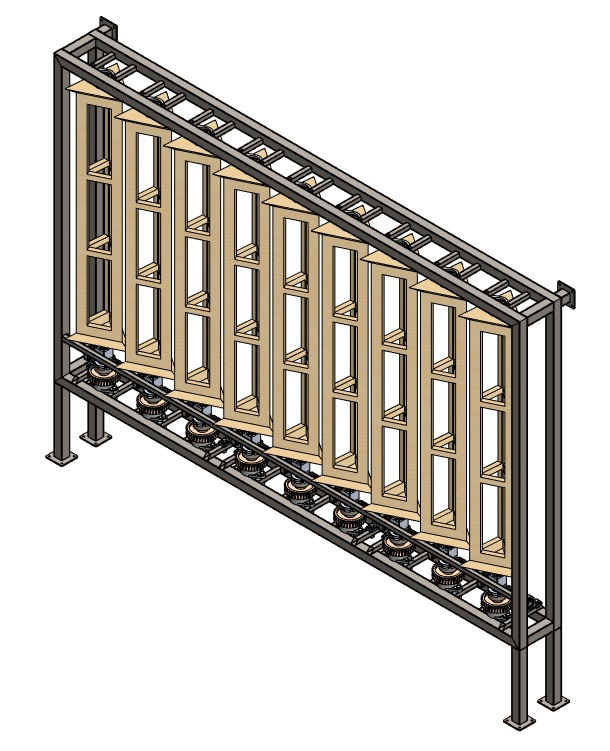
\includegraphics[width=1\textwidth]{imagenes/ConceptoSolucion.jpg}
    \caption{\footnotesize Concepto solución elegido}
    \label{fig:ConceptoSolucionElegido}
\end{figure}
\FloatBarrier
%------------------------------Elegido----------------------------------

\input{Secciones/Media 2/DiseñoDetallado}

\section*{Administración del proyecto}
\subsection*{Presupuesto estimado e infraestructura}
%tablas 5, 6 y 7 
%-----------------------------tabla 5-----------------------------
\begin{center}
\footnotesize
    \begin{longtable}[!htb]{| m{15em} | m{6em} | m{6em}| m{6em}|}
    \hline
    \textbf{Personal}& \textbf{\'Area de aporte} & \textbf{Instituci\'on} & \textbf{Tiempo m\'inimo}\\
    \hline\hline
    Estudiante: Barbosa Mercado José Aarón & STEM & UPIITA-IPN & 600 hrs\\
    \hline
    Estudiante: Camarena Rodríguez Alberto & STEM & UPIITA-IPN & 600 hrs\\
    \hline
    Estudiante: Muñoz Ceballos Teddy Xavier & STEM & UPIITA-IPN & 600 hrs\\
    \hline
    Estudiante: Sánchez Trujillo Daniel & STEM & UPIITA-IPN & 600 hrs\\
    \hline
    Asesor: Dr. Rafael Trovamala Landa & STEM & UPIITA-IPN/Ik'Atl & 60 hrs\\
    \hline
    Asesor: Dr. Alberto Luviano Juárez & STEM & UPIITA-IPN & 60 hrs\\
    \hline
    Especialista Externo: Rogelio Israel Quintero Tiscareño & Ingeniero en audio & Espiral Est\'ereo & 50 hrs\\
    \hline

    \caption{Tabla de recursos humanos.}
    \label{tab:RH}
    \end{longtable}
\end{center}
%-----------------------------tabla 5-----------------------------

%-----------------------------tabla 6-----------------------------
\begin{center}
\footnotesize
    \begin{longtable}[!htb]{| m{10em} | m{12em} | m{12em}|}
    \hline
    \textbf{Infraestructura}& \textbf{Desciripci\'on} & \textbf{Uso} \\
    \hline\hline
    Estudio de grabaci\'on & Recinto sobre el cual se desea hacer el tratamiento acústico. & Es el cuarto destinado sobre el que se trabajará el trabajo terminal.\\
    \hline
    Laboratorio de pesados & Taller donde se encuentran las máquinas e instrumentos. & En él, se manufacturarán las piezas.\\
    \hline

    \caption{Infraestructura para el desarrollo del proyecto.}
    \label{tab:Infraestructura}
    \end{longtable}
\end{center}
%-----------------------------tabla 6-----------------------------
%-----------------------------tabla 7-----------------------------
\begin{center}
\scriptsize
    \begin{longtable}[!htb]{| m{4em} | m{8em} | m{4.5em}| m{4em}| m{3em}| m{8em}| m{4em}|}
    \hline
    \textbf{M\'odulo}& \textbf{Material} & \textbf{Cantidad} & \textbf{Costo unitario} & \textbf{Costo total} & \textbf{Financiamiento} & \textbf{Fuente}\\
    \hline\hline
    \multirow{7}{*}{MMRP} 
    & Monitor de audio con amplificador & 1 & $\$$3,514 & $\$$3,514 & Privado & [20]\\
    \cline{2-7}
    & Micr\'ofono de condensador & 1 & $\$$3,599 & $\$$3,599 & Privado & [21]\\
    \cline{2-7}
    & Interfaz de audio & 1 & $\$$2,199 & $\$$2,199 & Privado & [22]\\
    \cline{2-7}
    & Cable XLR balanceado & 1 & $\$$167 & $\$$167 & Privado & [23]\\
    \cline{2-7}
    & Pedestal & 1 & $\$$188 & $\$$188 & Privado & [24]\\
    \cline{2-7}
    & Software generador de onda arbitraria & 1 & $\$$0 & $\$$0 & Privado & Estimado\\
    \cline{2-7}
    & Software para adquisici\'on de datos & 1 & $\$$0 & $\$$0 & Privado & Estimado\\
    \hline

    \multirow{5}{*}{MMP} 
    & Tarjeta de desarrollo & 1 & $\$$752 & $\$$752 & Propio & [25]\\
    \cline{2-7}
    & Motor & 4 & $\$$256 & $\$$1,024 & Propio & [26]\\
    \cline{2-7}
    & Panel ac\'ustico profesional de absorci\'on & 5 & $\$$673 & $\$$3,375 & Privado & [27]\\
    \cline{2-7}
    & Cople de uni\'on  & 4 & $\$$200 & $\$$800 & Propio & Estimado\\
    \cline{2-7}
    & Material de construci\'on de paneles de difusi\'on  y reflexi\'on (Madera) & 5 & $\$$385 & $\$$1,935 & Propio & [28]\\
    \hline

    & Esponja aislante & 5 & $\$$623 & $\$$3,115 & Propio & [29]\\
    \hline
    
    & Espuma absorbente & 5 & $\$$1,892 & $\$$9,460 & Propio & [30]\\
    \hline

    MCI & Software de control  & 1 & $\$$0 & $\$$0 & Privado & Estimado\\
    \hline
    MPC & Software de interfaz & 1 & $\$$0 & $\$$0 & Privado & Estimado\\
    \hline
    
    \caption{Presupuesto estimado}
    \label{tab:Presupuesto}
    \end{longtable}
\end{center}


%-----------------------------tabla 7-----------------------------
El costo total aproximado del proyecto sería $\$30,108$

\subsection*{Planeaci\'on de actividades}
\begin{figure}[!htb]
    \centering
    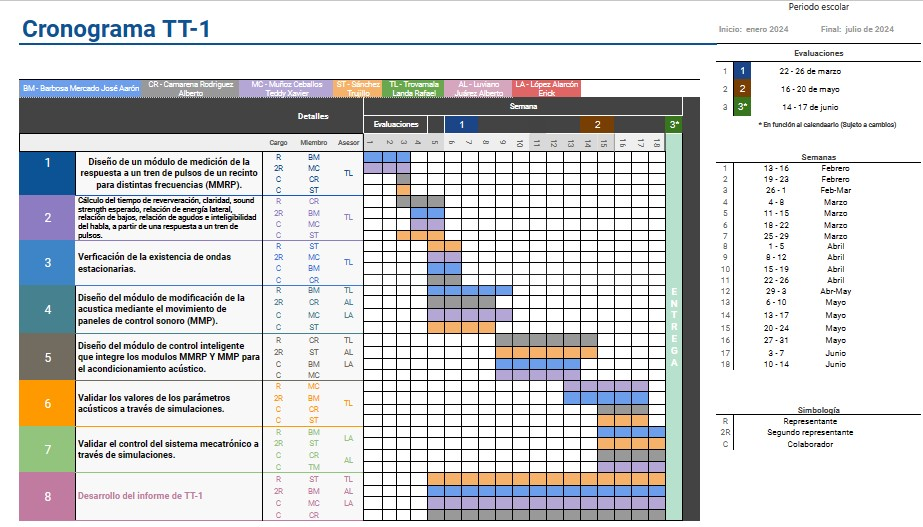
\includegraphics[width=1\textwidth]{imagenes/Protocolo21.jpg}
    \caption{\footnotesize Cronograma de actividades para TT1.}
\end{figure}
\FloatBarrier

\begin{figure}[!htb]
    \centering
    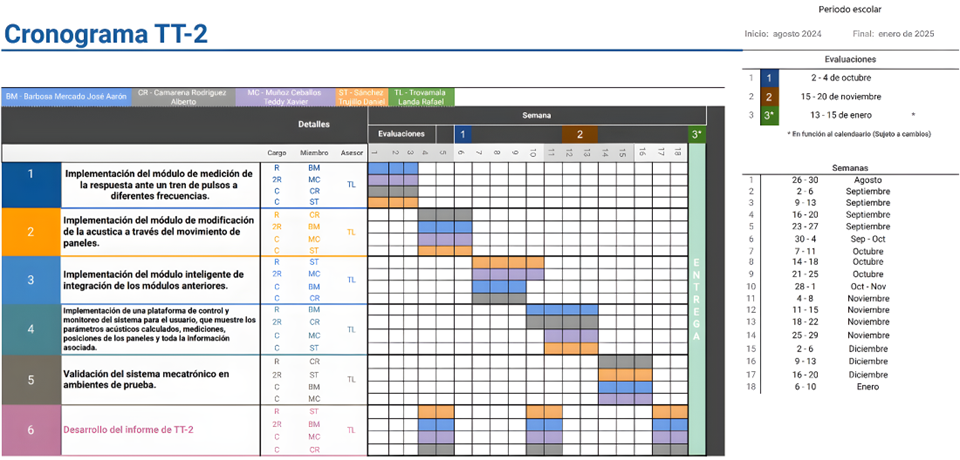
\includegraphics[width=1\textwidth]{imagenes/Protocolo22.png}
    \caption{\footnotesize Cronograma de actividades para TT2.}
\end{figure}
\FloatBarrier

%----------------------------------------------------
\input{Secciones/Adicional/Apéndices}


\section{Diseño del sistema}
\subsection{Diseño conceptual}
\subsubsection{Necesidades y requerimientos}
\subsubsection{Arquitectura funcional}
\subsubsection{Propuestas solución}

$S_{1}$: Sistema de medición de la acústica \\
\tab    $M_{1}$: Modulo de generación del tren de pulsos \\
\tab    $M_{2}$: Modulo de medición de la respuesta \\
\tab    $M_{3}$: Modulo de procesado y calculo \\
$S_{2}$: Sistema de control y procesado \\
$S_{3}$: Sistema de movimiento de paneles acústicos \\
$S_{4}$: Sistema de interfaz humano-maquina \\
\tab    $M_{4}$: Modulo de despliegue de información
$S_{5}$: Sistema de gestión de la energía \\

Se realizo una matriz de trazabilidad para verificar que los sistemas y módulos propuestos para la arquitectura física cumplieran con las funciones a ser desempeñadas.
%\bibliographystyle{ieeetr}
\selectlanguage{english}
\printbibliography
\selectlanguage{spanish}


\end{document}
